\documentclass[output=paper]{langsci/langscibook} 
\ChapterDOI{10.5281/zenodo.5040314}

\author{Ana-Sabina Uban\affiliation{Human Language Technologies Research Center, University of Bucharest; PRHLT Research Center, Universitat Politècnica de València} and
Alina Maria Ciobanu\affiliation{Human Language Technologies Research Center, University of Bucharest} and
Liviu P. Dinu\affiliation{Human Language Technologies Research Center, University of Bucharest}}
\title{Cross-lingual laws of semantic change}

\abstract{Semantic divergence in related languages is a key concern of historical linguistics. In order to complement existing research on semantic change, which in most previous approaches relies on the comparative analysis of diachronic corpora, we propose a novel approach for measuring semantic shifts synchronically. In this chapter, we investigate semantic change across languages by measuring the semantic distance of cognate sets using cross-lingual word embeddings.  We define a measure of cognate divergence and show how it can be used as a measure of language semantic divergence.
We propose an algorithm to detect and correct false friends as an application for natural language processing. We hypothesize that false friends fall on a spectrum, and define a corresponding notion of ``falseness'' and a methodology for its quantification. We evaluate the algorithm based on WordNet and on manually curated lists of true cognates and false friends, showing accuracy values exceeding 80\%, and we show how choosing a falseness level as a threshold for detecting false friends can affect the performance of the detection algorithm.
We further study the properties of the semantic divergence of cognates, and verify whether hypothesized laws of semantic change (namely the law of conformity and the law of innovation) hold in the multilingual setting, thus formulating the first laws of cross-lingual semantic change. We further study the mathematical relation between polysemy and frequency on the one hand, and falseness on the other hand, and identify polynomials that optimally model their relationship, leading to equations describing cross-lingual semantic change in relation to word properties.}

\begin{document}
\maketitle

\section{Introduction}
\label{section:introduction}

Semantic change -- that is, change in the meaning of individual words \citep{cognatesuban:campbell_1998} -- is a continuous, inevitable process stemming from numerous reasons and influenced by various factors. Words are continuously changing, with new senses emerging all the time. \citet{cognatesuban:campbell_1998} presents no less than 11 types of semantic change that are generally classified in two broad categories: narrowing and widening. The author states that most linguists found structural and psychological factors to be the main cause of semantic change, but the evolution of technology and cultural and social changes are not to be omitted.

Intra-lingual semantic shift has been previously studied in computational linguistics, but monolingual studies can only provide a limited picture of the evolution of word meanings, which often develop in a multilingual setting, with new words entering the language through inheritance and borrowing.
Measuring semantic divergence across languages can be useful in theoretical and historical linguistics -- being central to models of language and cultural evolution -- but also in downstream applications relying on cognates, such as machine translation.

\textsc{cognates} are words in sister languages (languages descending from a common ancestor) with a common proto-word. For example, the Romanian word \emph{victorie} and the Italian word \emph{vittoria} are cognates, as they both descend from the Latin word \emph{victoria} `victory' -- see Figure \ref{fig:cognates}. 
Cognates can help students when learning a second language and contribute to the
expansion of their vocabularies.
Cognate sets have also been used in a number of applications in natural language processing, including, for example, machine translation \citep{cognatesuban:zhao_and_zhang}. These applications rely on properly distinguishing between true cognates and false friends.

\begin{figure}
% % 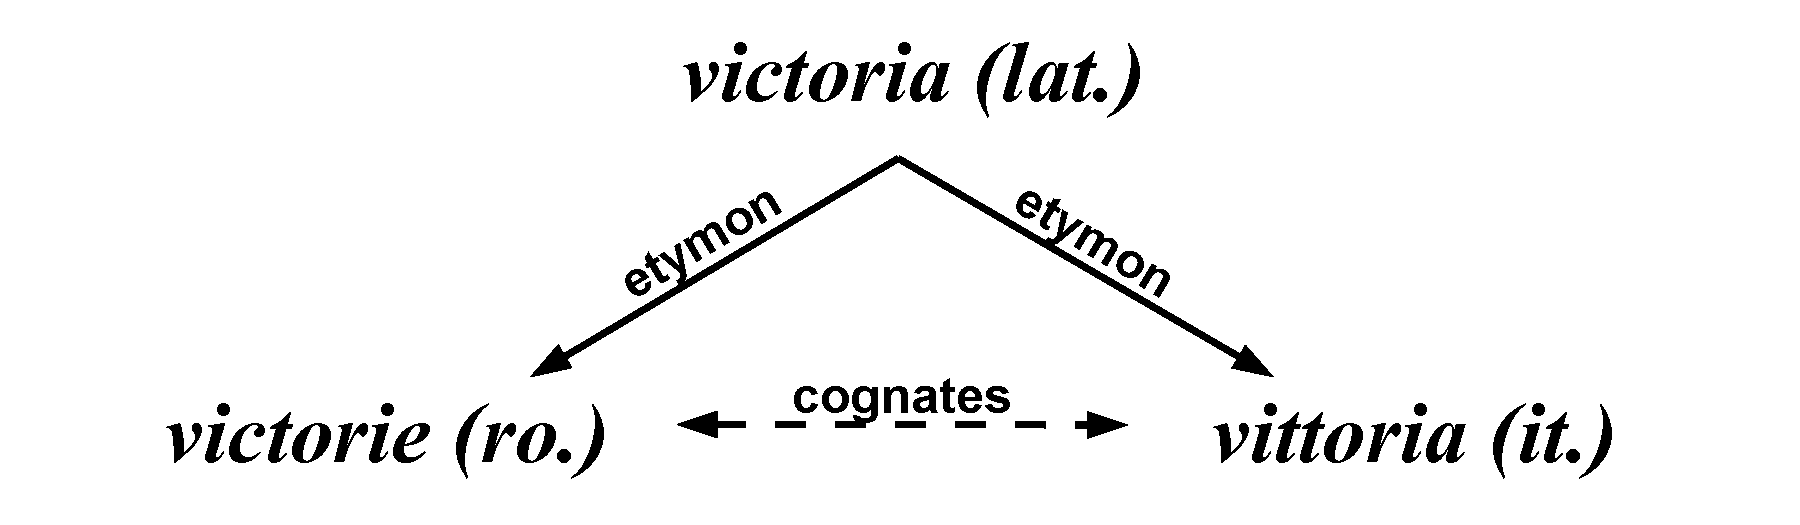
\includegraphics[width=200pt]{figures/UBAN_cognates_example.pdf}
\begin{forest}
[{\itshape victoria} (lat.), l sep=3\baselineskip, s sep=4.25cm
 [{\itshape victorie} (ro.), edge={-{Triangle[]}}, edge label={node[above,sloped,midway]{etymon}}, name=ro]
 [{\itshape vittoria} (it.), edge={-{Triangle[]}}, edge label={node[above,sloped,midway]{etymon}}, name=it]
]
\draw[<->,dashed,>=Triangle] (ro) -- (it) node[midway,above] {cognates};
\end{forest}
\caption{\label{fig:cognates}Example of cognates and their common ancestor.}
\end{figure}


In most cases, cognates have preserved similar meanings across languages, but there are also exceptions. In some cases, the meanings of cognates have diverged from the common etymon through their use in each of the two languages, and their meanings became different from each other. These are called \textit{deceptive cognates} or, more commonly, \textit{false friends}. Here we use the definition of cognates that refers to words with similar appearance and some common etymology, while \textit{true cognates} is used to refer to cognates which also have a common meaning, and \textsc{deceptive cognates} or \textsc{false friends} refers to cognate pairs which do not have the same meaning (anymore).

Many false friends have diverged into entirely different meanings. There are many examples, however, for which the changes in meaning are more subtle (for example, in connection with the feeling attached to a word or at the level of connotations) and more difficult to detect even for humans. The notion of semantic equivalence used to define false friends is in itself ambiguous and difficult to treat as a binary property, and we propose in this chapter that the quality of a cognate pair of being in a false friends relationship should also be treated as a spectrum. Based on this observation, we define the notions of \textsc{hard false friend} and \textsc{soft false friend}.

\textsc{hard false friends} are cognates whose meanings have diverged enough such that they do not have the same sense anymore, and should not be used interchangeably (as translations of one another). Most known examples of false friends fall in this category, such as the French-English cognate pair \textit{attendre}\slash\textit{at\-tend}: in French, \textit{attendre} has a completely different meaning, which is `to wait'. A different and more subtle type of false friends is represented by \textsc{soft false friends}, which can result from minor semantic shifts between the cognates. In such pairs, the meaning of the words may remain roughly the same, but with a difference in nuance or connotation. Such an example is the Romanian-Italian cognate pair \textit{amic}/\textit{amico}. Here, both cognates mean `friend', but in Italian the connotation is that of a closer friend, whereas the Romanian \textit{amic} denotes a more distant friend, or even acquaintance. A more suitable Romanian translation for \textit{amico} would be \textit{prieten}, while a better translation in Italian for \textit{amic} could be \textit{conoscente}. Though their meaning is roughly the same, translating one word for the other would be an inaccurate use of the language. These cases are especially difficult to handle by beginner language learners (especially since the cognate pair may appear as a valid translation in multilingual dictionaries). In these cases, instead of helping non-natives to more easily understand a text in a foreign language, cognates can instead cause more confusion and deceive the language learner into misunderstanding the text, as  using them in the wrong contexts is an easy trap to fall into.

Given these considerations, an automatic method for finding the appropriate term to translate a cognate into instead of using a false friend would be useful for assisting with language learning and text comprehension in a foreign language.
Moreover, identifying false friends can be useful not only for language acquisition, but also in downstream applications relying on cognates, such as machine translation.

\subsection{Related work}

Cross-lingual semantic word similarity consists in identifying words that refer to similar semantic concepts and convey similar meanings across languages \citep{cognatesuban:vulic_and_moens_2}. Some of the most popular computational approaches developed for this task rely on probabilistic models \citep{cognatesuban:vulic_and_moens} and cross-lingual word embeddings \citep{cognatesuban:soegard_et_al}. In this area, a fundamental task is that of Bilingual Lexicon Induction \citep{cognatesuban:mikolov2013exploiting,cognatesuban:heyman2017bilingual,cognatesuban:vulic-moens-2015-bilingual}, which aims to discover new translations at the lexical level by automatically mapping between vector spaces of languages.

A comprehensive list of cognates and false friends for every language pair is difficult to find or manually build. Moreover, dictionaries grow outdated and it is difficult to continuously update them to incorporate new words in the vocabulary. This is why applications have to rely on automatically identifying false friends.

There have been a number of previous studies attempting to automatically extract pairs of true cognates and false friends from corpora or from dictionaries. Most methods are based either on orthographic and phonetic similarity, or require large parallel corpora or dictionaries \citep{cognatesuban:inkpen2005automatic,cognatesuban:st2017identifying,cognatesuban:nakov2009unsupervised,cognatesuban:chen2016false}. 

\citet{cognatesuban:inkpen2005automatic} use orthographic features to extract French-English cognate pairs, but do not take semantic similarity into account. \citet{cognatesuban:torres2011using} also rely on orthographic and phonetic features, to which they add a semantic feature extracted from a bilingual dictionary. They additionally release a lexicon of Spanish-Portuguese false friends and true cognates, obtained through manual annotation, that they use to evaluate their algorithms.
\citet{cognatesuban:nakov2009unsupervised} identify false friends pairs in Bulgarian and Russian by making use of sentence-aligned parallel corpora. \citet{cognatesuban:aminian-etal-2015-unsupervised} propose using a model of identifying false friends from parallel corpora in order to improve English-Egyptian statistical machine translation.

There have been few previous studies using word embeddings for the detection of false friends or cognate words, usually using simple methods on only one or two pairs of languages \citep{cognatesuban:castro2018high,cognatesuban:torres2011using}. \citet{cognatesuban:castro2018high} detect false friends in Spanish-Portuguese, employing a classifier that learns from features extracted from multilingual embedding spaces.
\citet{cognatesuban:mitkov2007methods} use a method based on distributed representations of words in a continuous space built using comparable corpora, as well as a taxonomy-based approach, to identify false friends in four language pairs involving English, French, German and Spanish.\largerpage[-1]

In recent years, multiple computational linguistic studies have focused on the issue of semantic change, tracking the shift in the meaning of words by looking at their usage across time in corpora dating from different time periods. More than this, computational linguists have also tried to systematically analyze the principles describing semantic change hypothesized by linguists (such as the law of parallel change and the law of differentiation; \citealp{xu15}), or even proposed new statistical laws of semantic change, based on empirical observations, such as the law of conformity (stating that polysemy is positively correlated with semantic change), the law of innovation (according to which word frequency is negatively correlated with semantic change; \citealp{hamilton-etal-2016-diachronic}), or the law of prototypicality (according to
which prototypicality is negatively correlated
with semantic change; \citealp{dubossarsky2015bottom}).
More recently, \citet{dubossarsky-etal-2017-outta} revisited some of the semantic change laws proposed in previous literature, claiming that a more rigorous consideration of the control conditions when modelling these laws leads to the conclusion that they are weaker or less reliable than reported. More extensive surveys of computational studies relating to semantic change have been conducted by \citet{kutuzov-etal-2018-diachronic} and \citet{tahmasebi2018survey} (see also \citealp{chapters/01}).

All previous computational studies on lexical semantic change have, to our knowledge, only looked at the semantic change of the words in monolingual settings, and where more than one language was included, they were considered independently \citep{hamilton-etal-2016-diachronic}. However, words do not evolve only in their own language in isolation, but are rather inherited and borrowed between and across languages.
\citet{cognatesuban:dominguez2002false} distinguish between \textit{chance false friends}, which have similar form but different etymologies as well as different meanings in different languages, and \textit{semantic false friends}, which share the etymological origin, but their meanings differ (to some extent) in different languages. In this study we focus on the latter, which we consider more relevant from the point of view of semantic change since, in principle, they begin with a common meaning then diverge, to a lower or higher degree, while often preserving some common meaning, whereas \textit{chance false friends} usually have entirely distinct meanings.\largerpage[-1]

\begin{sloppypar}
\citet{cognatesuban:uban2019cognates} propose a method for identifying and correcting false friends and define a measure of their ``falseness'', using cross-lingual word embeddings. We base our study on the method proposed there and take it further by analyzing the properties of semantic divergence as they relate to different properties of the words, across five Romance languages, as well as English. Similarly to how \citet{hamilton-etal-2016-diachronic} formulate statistical laws of semantic change within one language, describing how word properties affect semantic change, we propose studying analogous laws cross-lingually, from the point of view of cognate divergence, studying this time the effect of semantic divergence on the subsequent evolution of the words, including properties such as frequency and polysemy. 
When a word enters a new language, features specific to that particular language (such as existing words in the same language or socio-cultural and historical factors) can affect the way it is used and contribute to shaping its meaning through time. The evolution of cognate words in different languages can be seen as a collection of different parallel histories of the proto-word from its entering the new languages to its current state.
Based on this view, we propose a novel approach for studying semantic change: instead of comparing \textit{monolingual} texts from \textit{different time periods} as ways to track meanings of words at different stages in time, we compare \textit{present meanings} of cognate words across \textit{different languages}, viewing them as snapshots in time of each of the word's different histories of evolution. We expand upon the work published in \citet{uban-etal-2019-studying} and continue exploring how properties (namely frequency and polysemy) of the words involved in semantic change relate to the degree of their semantic shift, and find the concrete mathematical functions that best describe the relationship. Additionally, we present examples of true cognates for each language (words which kept their Latin meaning in the modern language), and cluster them into semantic fields, which might provide some insight into the socio-cultural factors that are connected to semantic change.
\end{sloppypar}

\subsection{Contributions}
\begin{sloppypar}
The contributions of our work on cognate divergence are threefold. Firstly, we propose a method for quantifying the semantic divergence of languages. Secondly, we provide a framework for detecting and correcting false friends, based on the observation that these are usually deceptive cognate pairs: pairs of words that once had a common meaning, but whose meaning has since diverged. Thirdly, we propose a novel way to measure semantic change synchronically across languages, by tracking the divergence of cognate words from their original etymon.
\end{sloppypar}

In Section~\ref{section:semantic-divergence}, we introduce a method for measuring the semantic divergence of sister languages based on cross-lingual word embeddings. We use a multilingual set of cognates extracted from etymology dictionaries and word embeddings trained on Wikipedia corpora. By comparing current meanings of cognate sets in different languages, our method can uncover insights about how their meanings diverged within their respective languages from their common original etymon, and infer properties of the parallel processes of change in the meaning of cognate words across time. We report empirical results on five Romance languages: Romanian, French, Italian, Spanish and Portuguese. For a deeper insight into the matter, we also compute and investigate the semantic similarity between modern Romance languages and Latin. We then introduce English into the mix, to analyze the behavior of a more remote language, where words deriving from Latin are mostly borrowings. We show that, in terms of semantic divergence, the studied languages form clusters that are consistent with the generally accepted tree of languages.
Moreover, we perform a qualitative analysis of the subset of cognates for which meaning was preserved from the etymon to the modern word, comparatively between different language pairs, and show how the original Latin meaning of words was preserved across Romance languages for different semantic fields. In Section~\ref{section:false-friends}, we propose a fully automated, unsupervised method for false friend detection and correction, relying on cross-lingual word embeddings. We propose a corpus-based approach that is capable of covering the majority of the vocabulary for a large number of languages, while at the same time requiring minimal human effort in terms of manually evaluating word pair similarity or building lexicons, relying only on large monolingual corpora.
We propose a method that can be used to identify pairs of false friends, to distinguish between the two categories of false friends defined above (\textit{hard false friends} and \textit{soft false friends}), and to provide suggestions for correcting the erroneous usage of a false friend in translation. We evaluate the algorithm on Romance languages and English. We build a dataset of false friends, publicly available, along with falseness scores for each pair.
In Section~\ref{section:laws-of-semantic-change}, we propose a method for measuring and characterizing semantic change using the semantic divergence of cognate sets. Building on related literature in computational linguistics, we study how laws of semantic change manifest cross-linguistically, trying to understand how semantic divergence affects word properties in the multilingual setting, from a reversed perspective compared to previous studies: namely measuring the effect of semantic change on word properties (such as frequency and polysemy). We show that, from this perspective, semantic divergence is positively correlated with both polysemy and frequency. 
In Section~\ref{section:conclusions}, we draw conclusions and discuss future work.

\subsection{Cross-lingual word embeddings}

Word embeddings are vectorial representations of words in a continuous space, built by training a model to predict the occurrence of a word in a text corpus, given its context, or the context, given the word. Based on the distributional hypothesis stating that similar words occur in similar contexts, these vectorial representations can be seen as semantic representations of words and can be used to compute semantic similarity between word pairs (representations of words with similar meanings are expected to be close together in the embedding space).

To compute the semantic divergence of cognates across sister languages, as well as to identify pairs of false cognates (pairs of cognates with high semantic distance), which by definition are pairs of words in two different languages, we need to obtain a multilingual semantic space, which is shared between the cognates. Having the representations of both cognates in the same semantic space, we can then compute the semantic distance between them using their vectorial representations in this space. Our research is related, in terms of methodology, to Bilingual Lexicon Induction, which has been extensively studied in previous research \citep{cognatesuban:mikolov2013exploiting,cognatesuban:heyman2017bilingual}, but in our case, we rely on inferred cross-lingual lexical semantic similarities in order to verify whether cognate pairs share the same meaning, rather than discover new translations.

For our purposes, we use the publicly available FastText \citep{bojanowski2017enriching} multilingual word embeddings, pre-trained on Wikipedia for the six languages in question, and pre-aligned in a common vector space \citep{cognatesuban:conneau2017word}.\footnote{\url{https://github.com/facebookresearch/MUSE}} The vectors have 300 dimensions and were obtained using the skip-gram model described by \citet{bojanowski2017enriching} with default parameters.

The algorithm for measuring the semantic distance between cognates in a pair of languages (\textit{lang1}, \textit{lang2}) consists of the following steps:\largerpage

\begin{enumerate}
\item Obtain word embeddings for each of the two languages.
\item Obtain a shared embedding space, common to the two languages. This is accomplished using an alignment algorithm, which consists of finding a linear transformation between the two spaces, that on average optimally transforms each vector in one embedding space into a vector in the second embedding space, minimizing the distance between a few seed word pairs (for which it is known that they have the same meaning), based on a small bilingual dictionary. For our purposes, we use the publicly available multilingual alignment matrices that were published by \citet{align_4}.
\item Compute semantic distances for each pair of cognate words in the two languages, using a vectorial distance (we chose cosine distance) on their corresponding vectors in the shared embedding space.
\end{enumerate}


When interpreting results based on aligned embedding spaces to infer conclusions on linguistic phenomena at the language level, various limitations of the method should be kept in mind, including biases due to the corpus used to train the embeddings, to the algorithm used to train the embeddings, or to the alignment operation. Unsupervised alignment of pre-trained monolingual embedding spaces for obtaining multilingual representations has been shown in previous studies to introduce noise in the resulting multilingual space \citep{cognatesuban:sogaard2018limitations,cognatesuban:beinborn2019semantic,cognatesuban:patra2019bilingual}, due to the simplifying assumptions on the isomorphy of monolingual embedding spaces, and to properties of the monolingual spaces themselves, leading to different alignment quality for different language pairs.
We attempt to minimize the effect of the confounding factors through our particular methodological choices, where possible, and through experiments designed to measure the contribution of the different factors in isolation.\largerpage[-1]


We choose the FastText \citep{bojanowski2017enriching} embeddings pre-trained on Wikipedia since they are trained on large amounts of text, which minimizes the amount of noise in the vectors, making them good approximators of word meanings. Additionally, they are trained on text that is relatively uniform in style and topic, which ensures that any difference in the structure of the embedding spaces of different languages depends on the language, rather than being an artifact of topic or genre. Nevertheless, even high quality embeddings can be noisy or biased and this should be kept in mind when interpreting the results of our experiments. Moreover, the uniformity of the writings in the corpus in terms of style and period of history when they were written can act as a weakness, limiting the embeddings' representativeness of the language as a whole \citep{koplenig2016}. For Latin in particular, we note that using Latin Wikipedia as a training corpus might bias representations away from the original usages of the words in Latin, and towards their usages in the modern languages the articles were translated from.

The algorithm that we use for computing semantic distance for cognate pairs stands on the assumption that the (shared) embedding spaces are comparable, so that the averaged cosine similarities and the overall distributions of scores that we obtain for each pair of languages can be compared in a meaningful way. For this to be true, at least two conditions need to hold:

\begin{enumerate}
\item The embedding spaces for each language need to be similarly representative of the language, or trained on similar texts -- this assumption holds sufficiently in our case, since all embeddings (for all languages) are trained on Wikipedia, which at least contains a similar selection of texts for each language, and at most can be considered comparable corpora.

\item The similarity scores in a certain (shared) embedding space need to be sampled from a similar distribution. To confirm this assumption, we compare distributions of a random sample of similarity scores across all embedding spaces. For each multilingual embedding space (corresponding to a language pair), we select at random 1,000,000 word pairs, and compute their similarities. We find that the similarity distributions are similar in mean and standard deviation across aligned embedding spaces, with mean similarity scores ranging between $(0.188, 0.199)$ for all language pairs, and all standard deviations between $(0.074, 0.082)$. On our (large) samples of word pairs used in this analysis, statistical t-tests show significant $(p < 0.05)$ difference between means across language pairs, but the effect is small: Cohen's d-test shows an effect size smaller than $0.09$ for all language pairs.

The observed consistency of word similarities across language pairs was not obvious but also not surprising, since:
\begin{itemize}\sloppy
    \item The way we create shared embedding spaces is by aligning the embedding space of any language to the English embedding space (which is a common reference to all shared embedding spaces).
    \item The nature of the alignment operation (consisting only of rotations and reflections) guarantees monolingual invariance, as described by \citet{cognatesuban:artetxe2016learning} and \citet{align_4}.
\end{itemize}
\end{enumerate}


\section{The semantic divergence of cognates}
\label{section:semantic-divergence}

We propose a definition of semantic divergence between two languages based on the semantic distances of their cognate word pairs in embedding spaces. The semantic distance between two languages can then be computed as the average semantic divergence of all pairs of cognates in that language pair.

As our data source for cognate words, we use the list of cognate sets in Romance languages proposed by \citet{cognatesuban:ciobanu_and_dinu_lrec}. It contains 3,218 complete cognate sets in Romanian, French, Italian, Spanish and Portuguese, along with their Latin common ancestors. The cognate sets are obtained from electronic dictionaries which provide information about the etymology of the words. Two words are considered cognates if they have the same etymon (i.e., if they descend from the same word). A subset of 305 of these sets also contains the corresponding cognate (in the broad sense, since these are mostly borrowings) in English.

One complete example of a cognate set for the word \textit{architect} in the Romance languages is illustrated in Table \ref{tab:cognate_set}.

\begin{table}
    \fittable{\begin{tabular}{cccccc}    \lsptoprule
    Romanian & French & Italian & Spanish & Portuguese & Latin ancestor \\\midrule
arhitect & architecte & architetto & arquitecto & arquiteto &    architectus \\
    \lspbottomrule
    \end{tabular}}
    \caption{An example of a cognate set: \textit{architect} in Romance languages.}
    \label{tab:cognate_set}
\end{table}

\subsection{The Romance languages}

We compute the cosine similarity between cognates for each pair of modern languages, and between modern languages and Latin as well. We compute an overall score of similarity for a pair of languages as the average similarity for the entire dataset of cognates. The results are reported in Table \ref{table:cognate_divergence}.

\begin{table}
\begin{center}
\begin{tabular}{l l l l l l}
\lsptoprule
& Fr & It & Pt & Ro & La\\
\midrule

Es & 0.67 & 0.69 & 0.70 & 0.58 & 0.41\\
Fr & & 0.66 & 0.64 & 0.56 & 0.40 \\
It & & & 0.66 & 0.57 & 0.41 \\
Pt & & & & 0.57 & 0.41\\
Ro & & & & & 0.40 \\
\lspbottomrule

\end{tabular}
\end{center}
\caption{\label{table:cognate_divergence}Average cross-lingual similarity between cognates (Romance languages).}
\end{table}


We observe that the highest similarity is obtained between Spanish and Portuguese (0.70), while the lowest values are obtained for Latin. From the modern languages, Romanian has, overall, the lowest degrees of similarity to the other Romance languages. A possible explanation for this result is the fact that Romanian developed far from the Romance kernel, being surrounded by Slavic languages. 
In Table \ref{table:similar_cognates} (page~\pageref{table:similar_cognates}) we report, for each pair of languages, the most similar (above the main diagonal) and the most dissimilar (below the main diagonal) cognate pair for Romance languages.



\begin{table}[p]
\fittable{\begin{tabular}{l l l l l l}
\lsptoprule
& Es & Fr & It & Ro & Pt \\
\midrule
Es & -- & ocho/ & diez/ & ocho/ & ocho/ \\
 & & huit (0.89) & dieci (0.86) & opt (0.82) & oito (0.89) \\
Fr & caisse/ & -- & dix/ & décembre/ & huit/ \\
 & casar (0.05) & & dieci (0.86) & decembrie (0.83) & oito (0.88) \\
It & prezzo/& punto/ & -- & convincere/ & convincere/ \\
& prez (0.06)  & ponte (0.09) & & convinge (0.75) & convencer (0.88) \\
Ro & miere/ & face/ & as/ & -- & opt/ \\
& mel (0.09) & facteur (0.10) & asso (0.11) & & oito (0.83) \\
Pt & prez/ & pena/ & preda/ & linho/ & --\\
 & preço (0.05) & paner (0.09) & prea (0.08) & in (0.05)  & \\
\lspbottomrule
\end{tabular}}
\caption{Most similar and most dissimilar cognates for all language pairs.\label{table:similar_cognates}}
\end{table}

The problem that we address in this experiment involves a certain \textit{vagueness of reported values} (also noted by \citealt{cognatesuban:eger_et_al} in the problem of semantic language classification), as there is no gold standard that we can compare our results to. To overcome this drawback, we use the degrees of similarity that we obtained to produce a language clustering, using the \textsc{unweighted pair group method with arithmetic mean} (UPGMA) hierarchical clustering algorithm \citep{cognatesuban:sokal_and_michener}. We observe that it is similar to the generally accepted tree of languages, and to the clustering tree built on intelligibility degrees by \citet{cognatesuban:ciobanu_and_dinu_intelligibility}. The obtained dendrogram is rendered in Figure \ref{fig:dendrogram_cognates}.

\begin{figure}[p]
\center
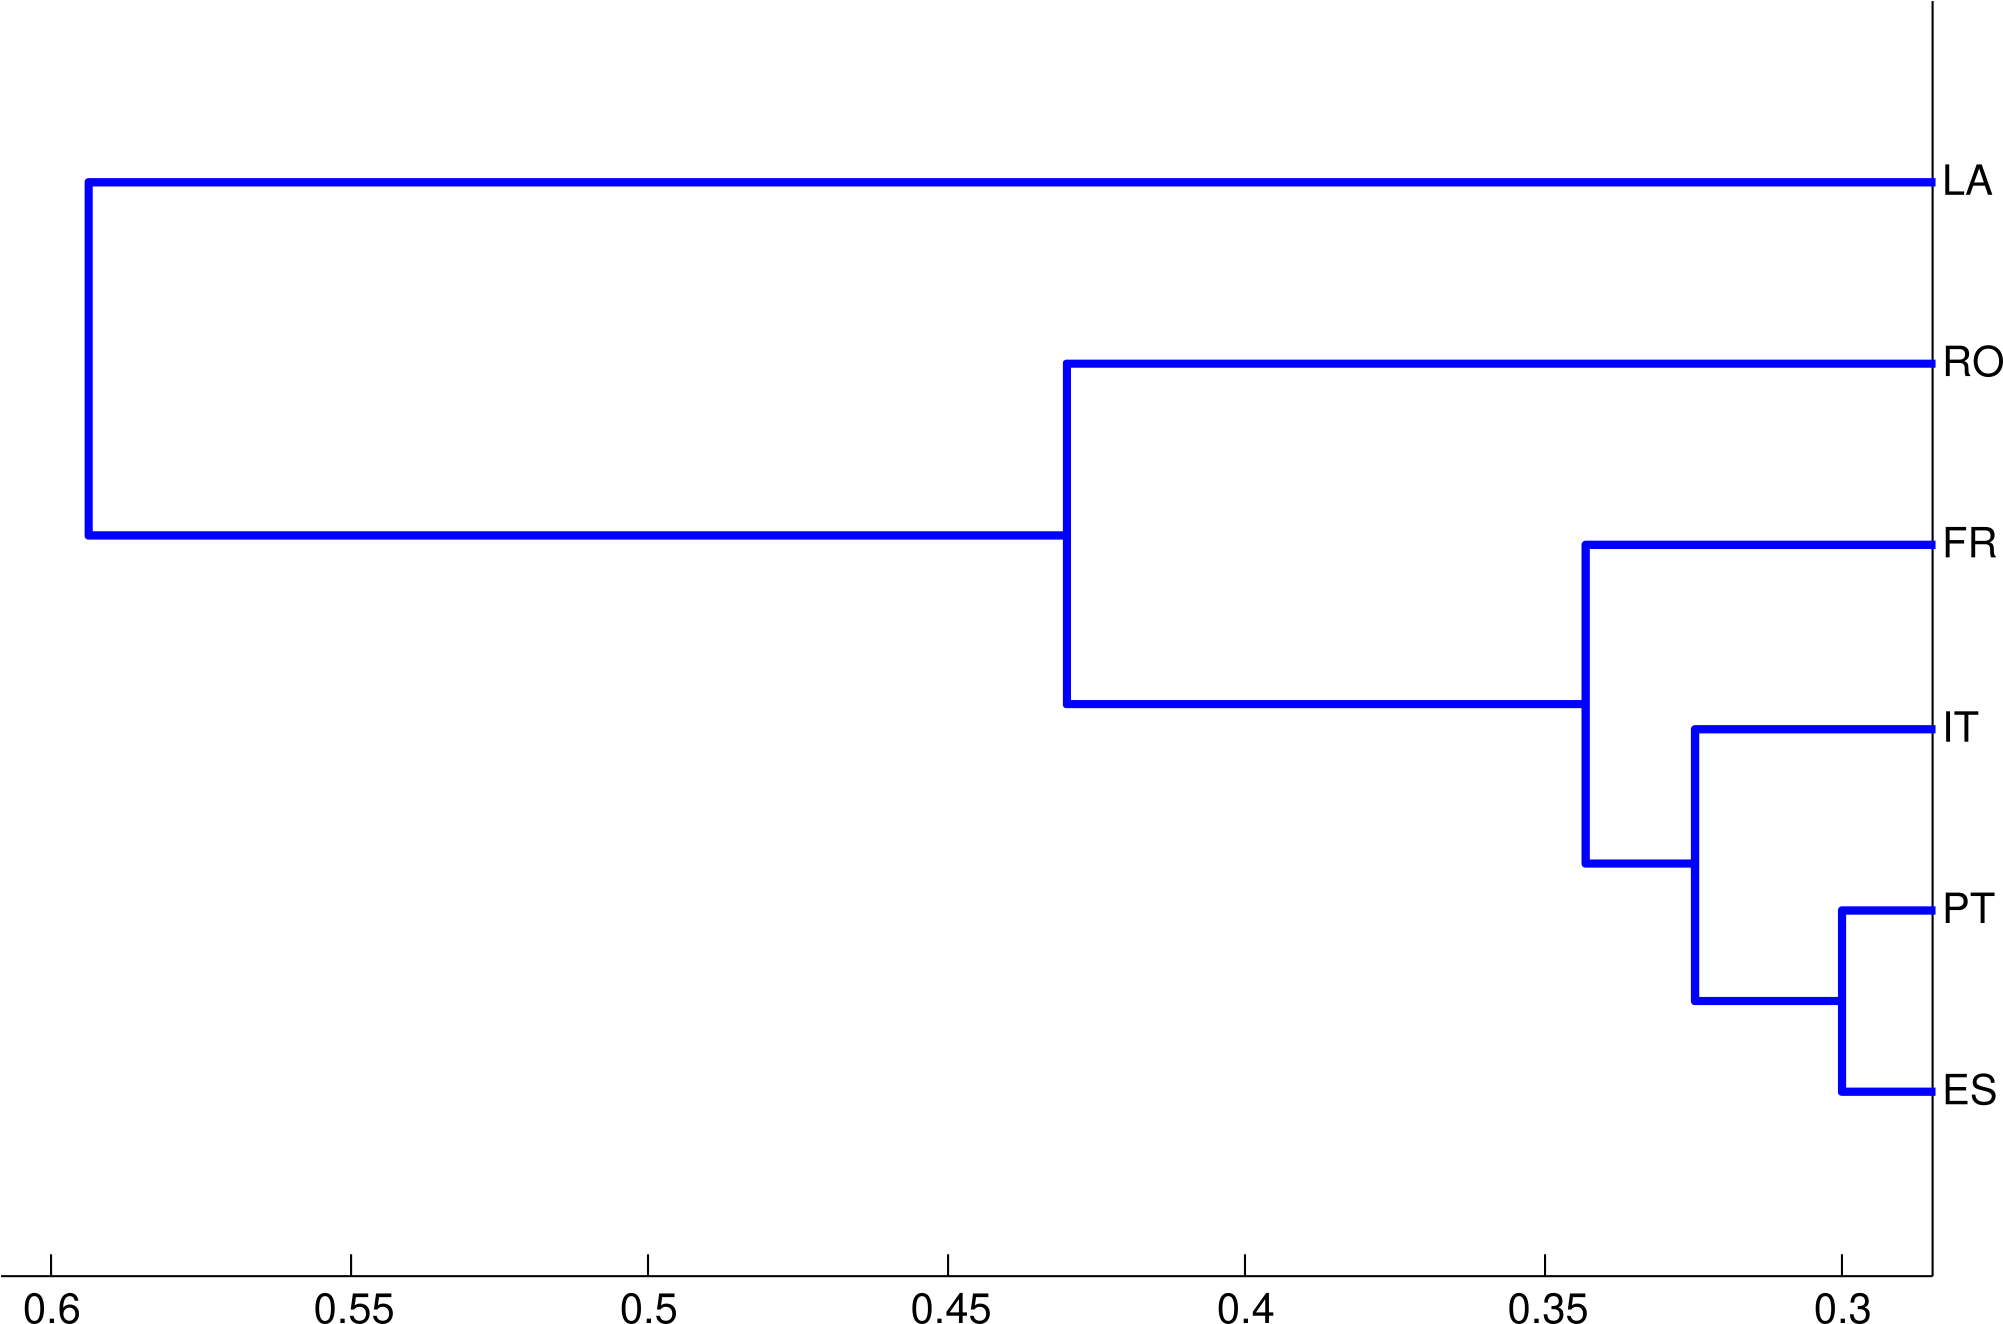
\includegraphics[width=0.8\linewidth]{figures/UBAN_dendrogram.png}
\caption{\label{fig:dendrogram_cognates}Dendrogram of the language clusters.}
\end{figure}

\subsection{The Romance languages vs. English}\largerpage

In this subsection, we introduce English into the mix. We run this experiment on a subset of the dataset of cognates, using only the words that have a cognate in English as well.\footnote{Here we ``stretch'' the definition of \emph{cognates}, as they are generally referring to sister languages. In this case English is not a sister of the Romance languages, and the words with Latin ancestors that entered English are mostly borrowings.} The subset has 305 complete cognate sets.

The results are reported in Table~\ref{table:cognate_similarity_en}, and the distribution of similarity scores for each pair of languages is rendered in Figure~\ref{fig:exp1}. We notice that English has a comparatively low similarity with Latin (0.40 similarity with Latin, the same as French and Romanian), but its cognates are close to the other languages. Out of the modern Romance languages, Romanian is the most distant from English, with 0.53 similarity.

\begin{table}[!ht]
\begin{center}
\begin{tabular}{l l l l l l l}
\lsptoprule
& Fr & It & Pt & Ro & En & La\\
\midrule

Es & 0.64 & 0.67 & 0.68 & 0.57 & 0.61 & 0.42 \\
Fr & & 0.64 & 0.61 & 0.55 & 0.60 & 0.40 \\
It & & & 0.65 & 0.57 & 0.60 & 0.41 \\
Pt & & & & 0.56 & 0.59 & 0.42 \\
Ro & & & & & 0.53 & 0.40 \\
En & & & & & & 0.40 \\
\lspbottomrule

\end{tabular}
\end{center}
\caption{\label{table:cognate_similarity_en}Average cross-lingual similarity between cognates.}
\end{table}


\begin{figure*}[!ht]
    \centering
    \begin{subfigure}{0.30\textwidth}
        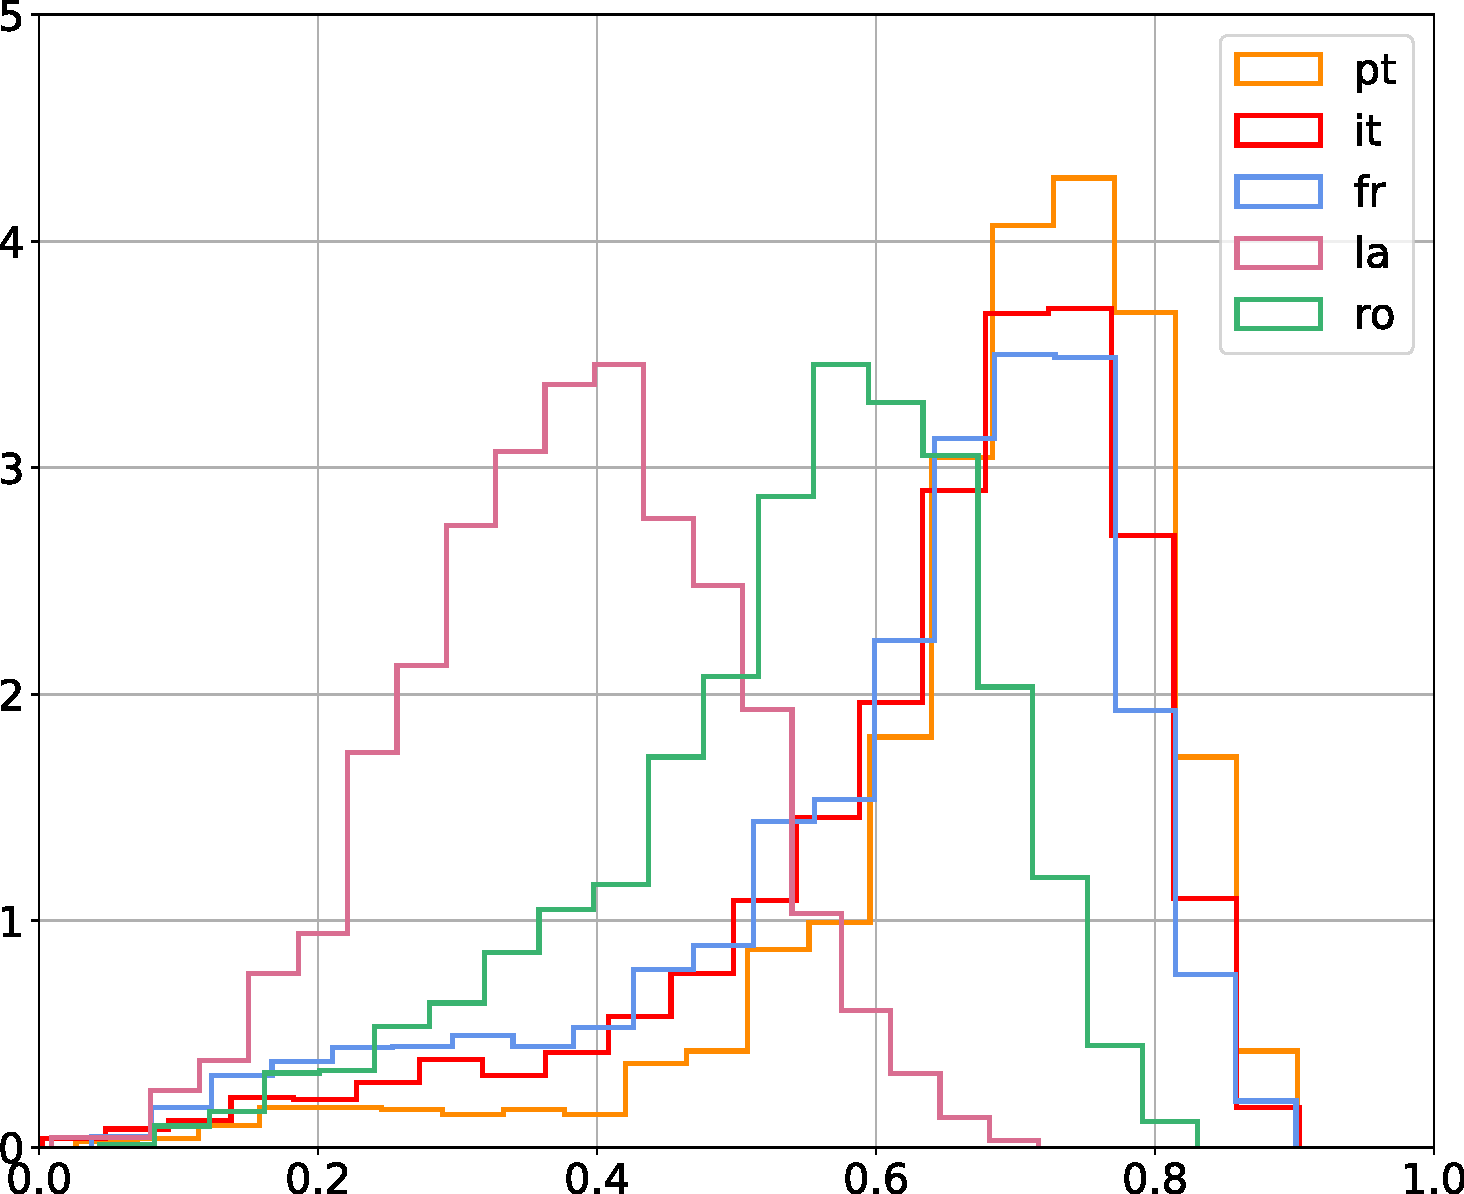
\includegraphics[width=\linewidth]{figures/UBAN_histogram_distances_es_all_contour.pdf}
        \caption{Spanish vs Romance}
    \end{subfigure}
    \begin{subfigure}{0.30\textwidth}
        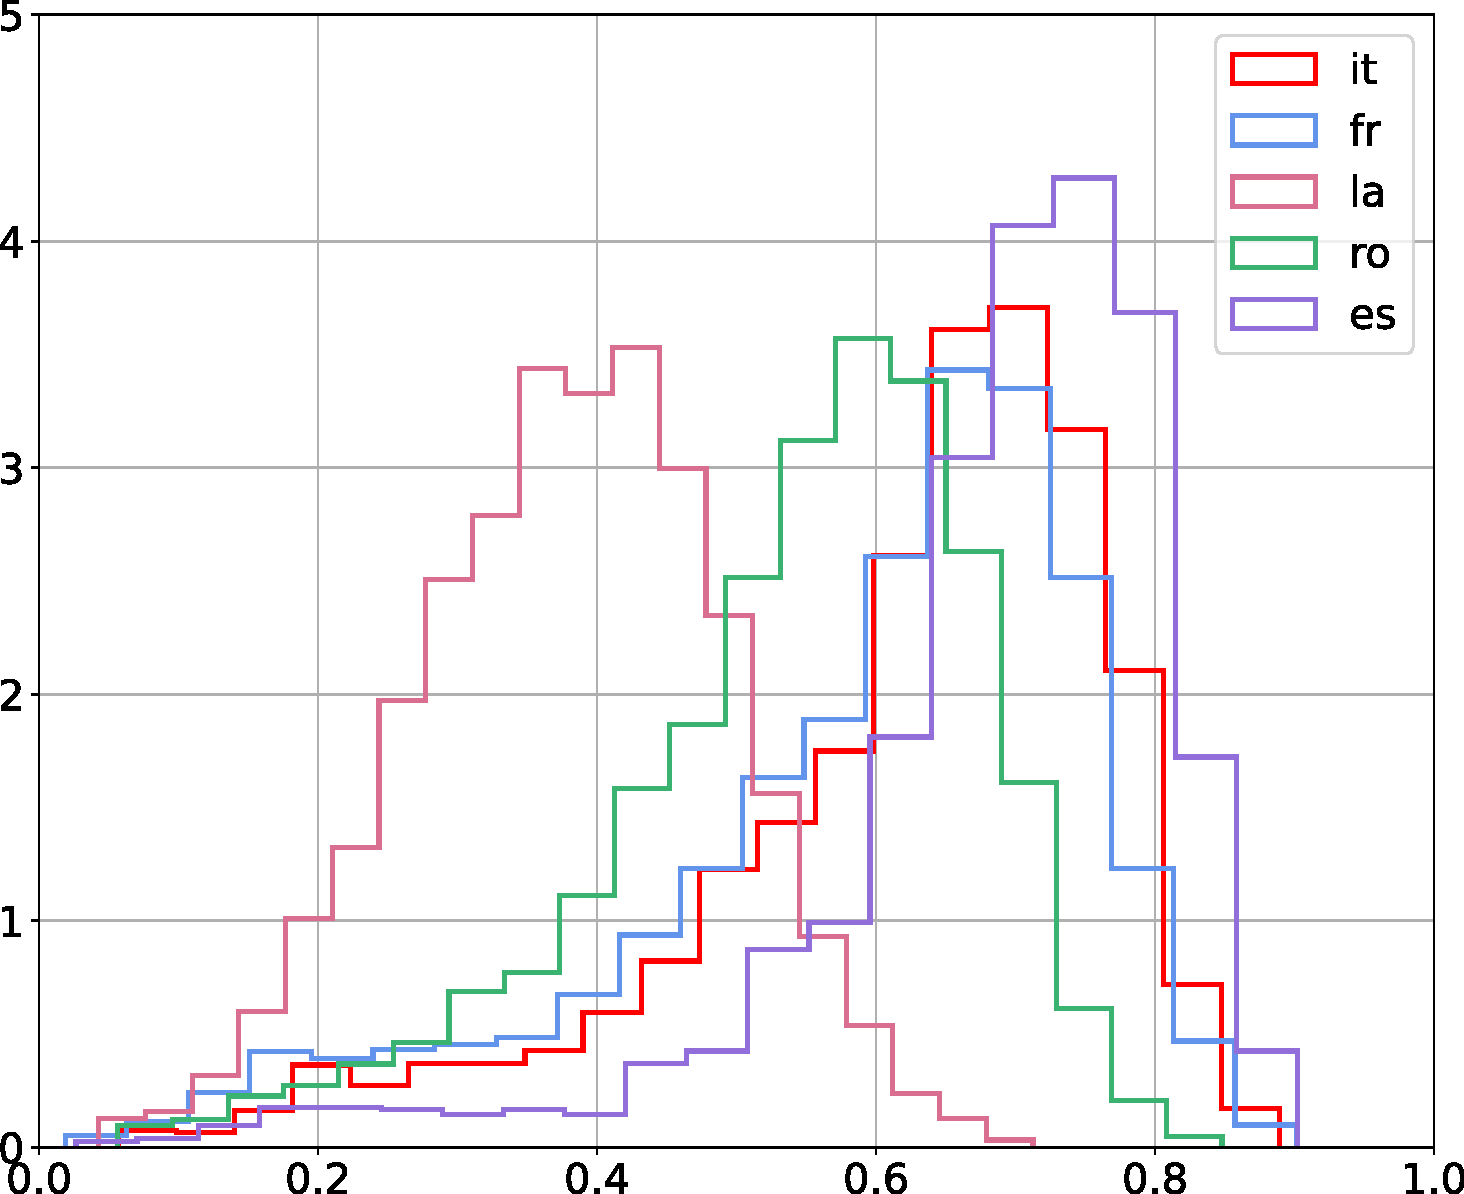
\includegraphics[width=\linewidth]{figures/UBAN_histogram_distances_pt_all_contour.pdf}
        \caption{Portuguese vs Romance}
    \end{subfigure}
    \begin{subfigure}{0.30\textwidth}
        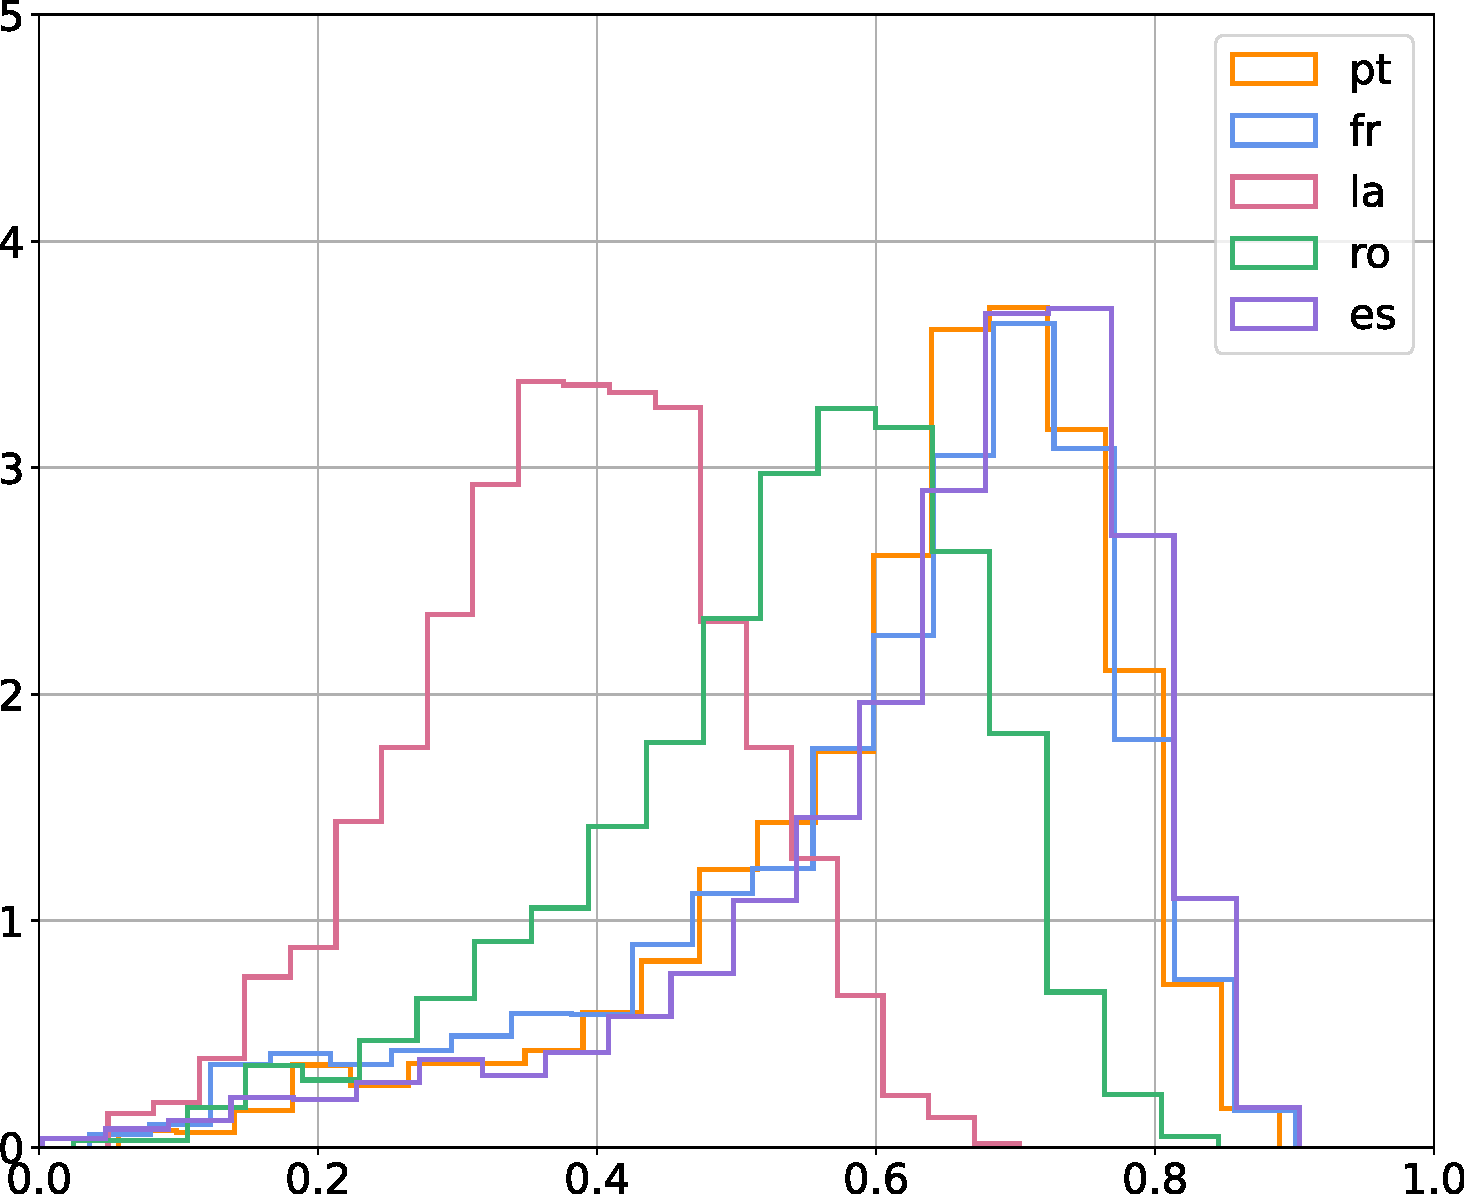
\includegraphics[width=\linewidth]{figures/UBAN_histogram_distances_it_all_contour.pdf}
        \caption{Italian vs Romance}
    \end{subfigure}
    \begin{subfigure}{0.30\textwidth}
        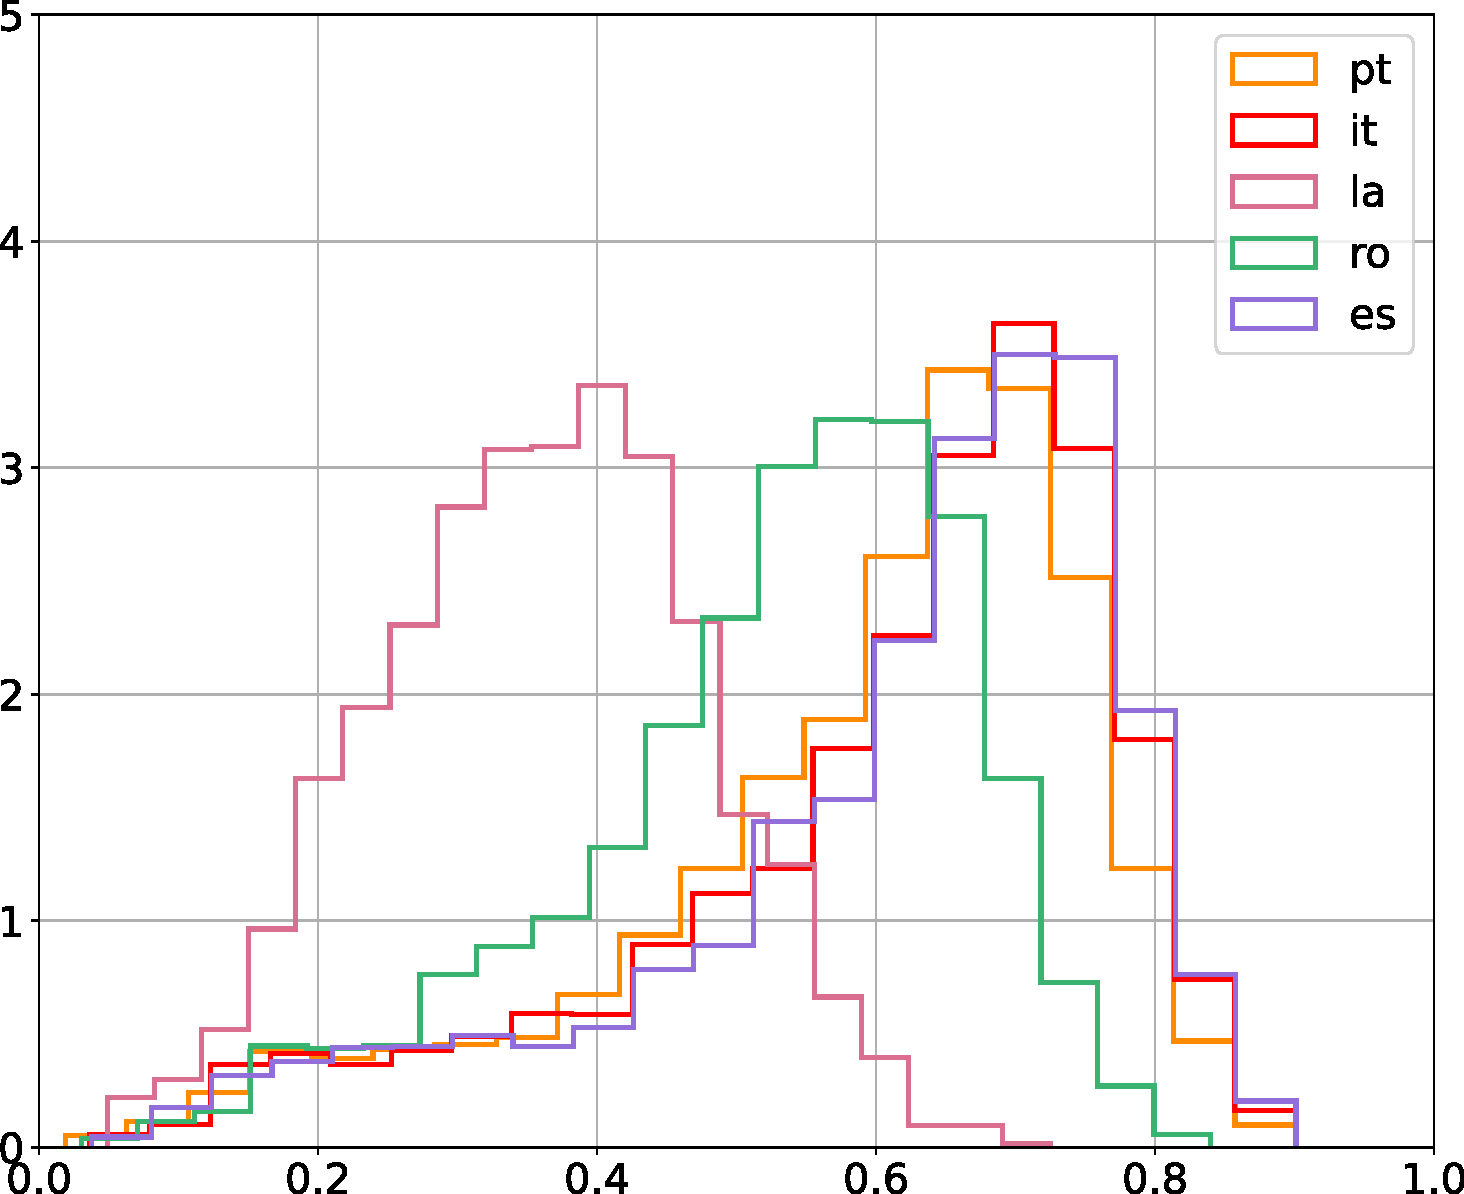
\includegraphics[width=\linewidth]{figures/UBAN_histogram_distances_fr_all_contour.pdf}
        \caption{French vs Romance}
    \end{subfigure}
    \begin{subfigure}{0.30\textwidth}
        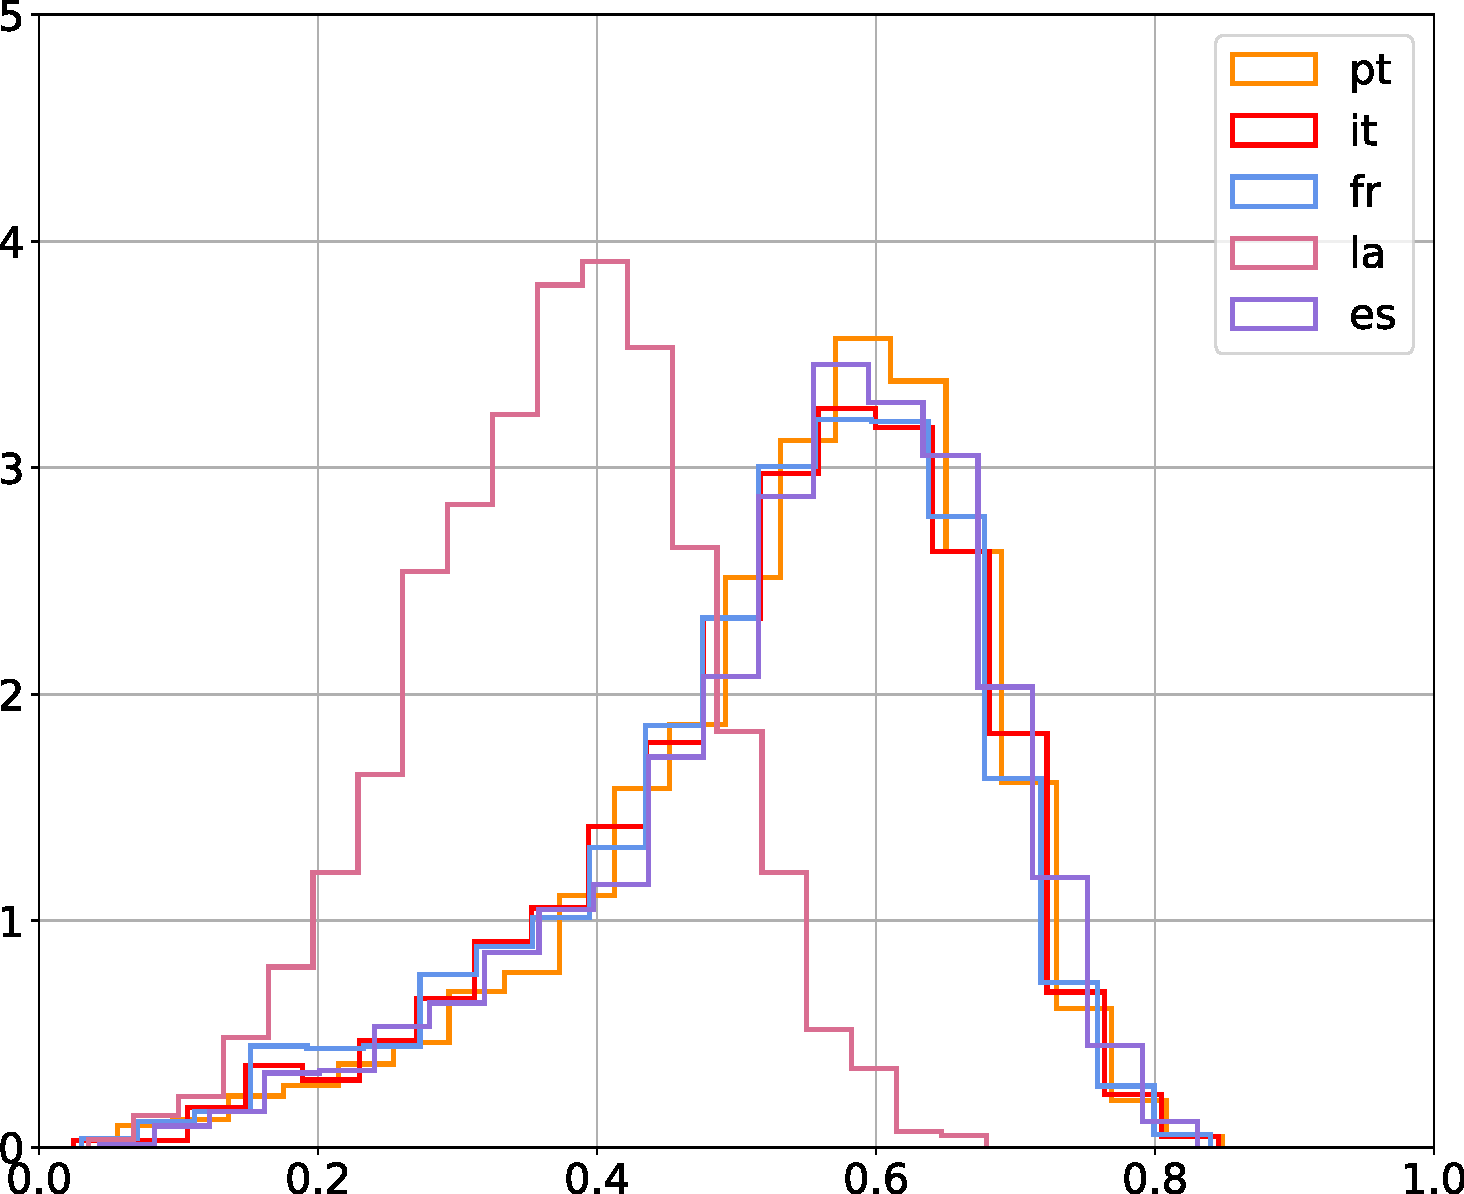
\includegraphics[width=\linewidth]{figures/UBAN_histogram_distances_ro_all_contour.pdf}
        \caption{Romanian vs Romance}
    \end{subfigure}
    \begin{subfigure}{0.30\textwidth}
        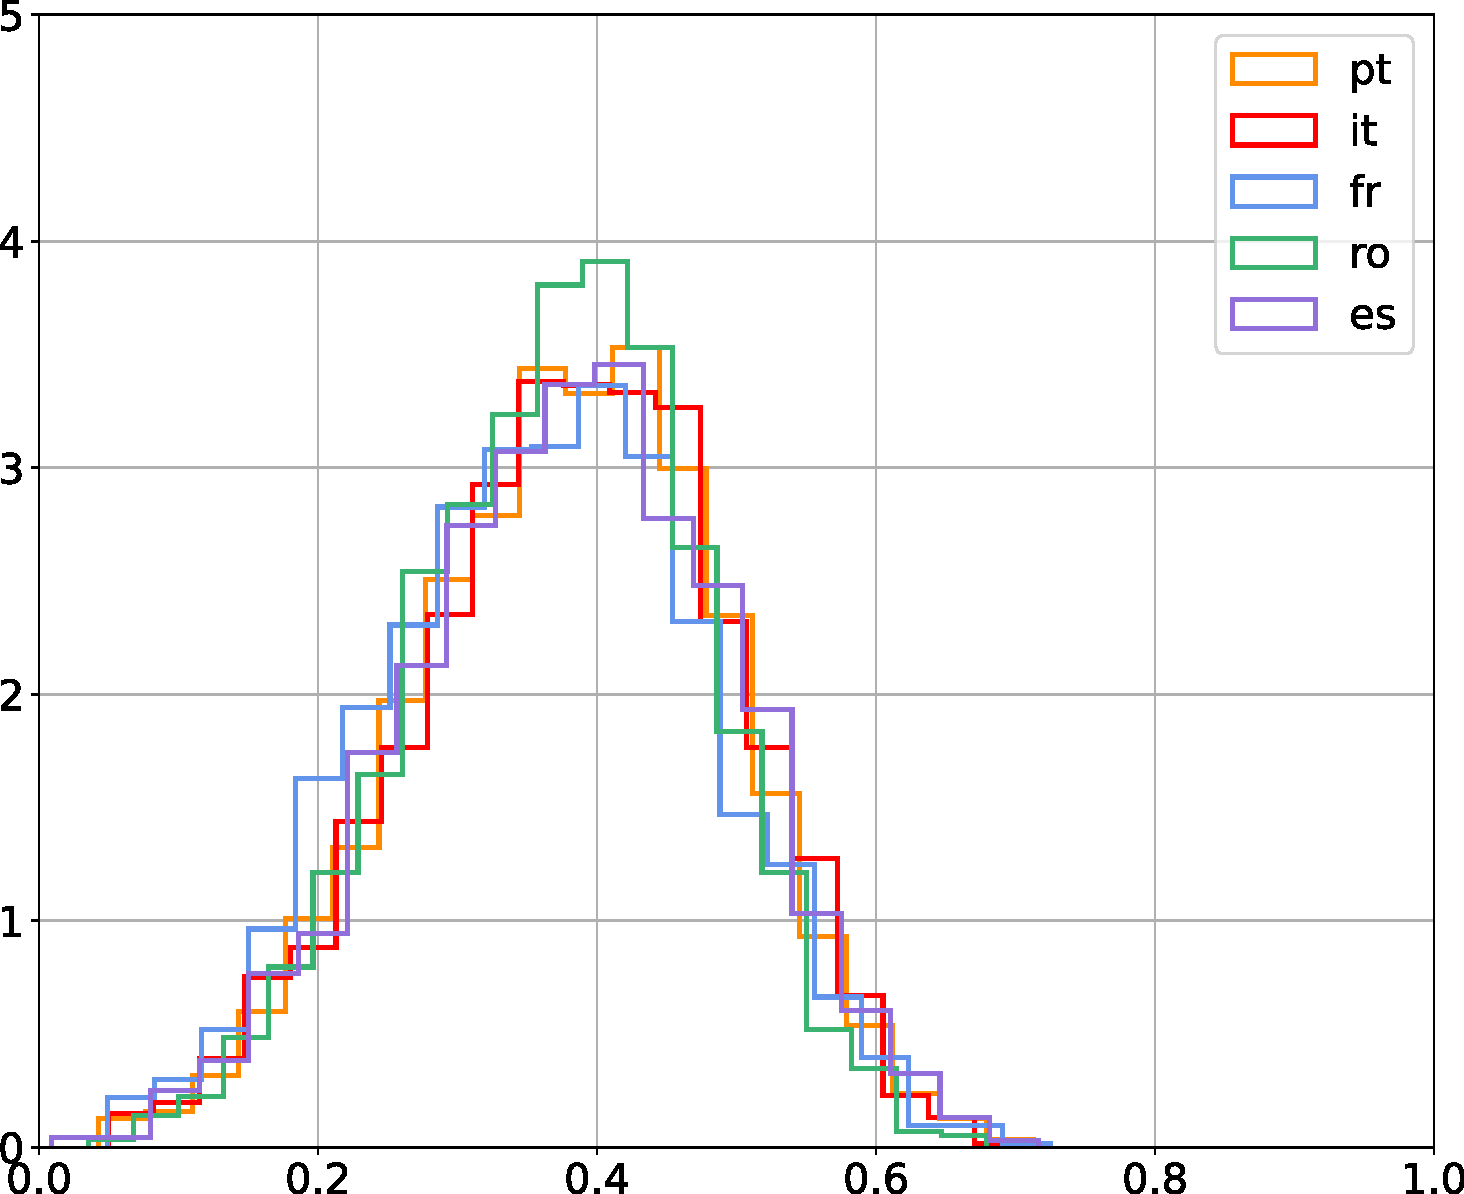
\includegraphics[width=\linewidth]{figures/UBAN_histogram_distances_la_all_contour.pdf}
        \caption{Latin vs Romance}
    \end{subfigure}
    \begin{subfigure}{0.30\textwidth}
        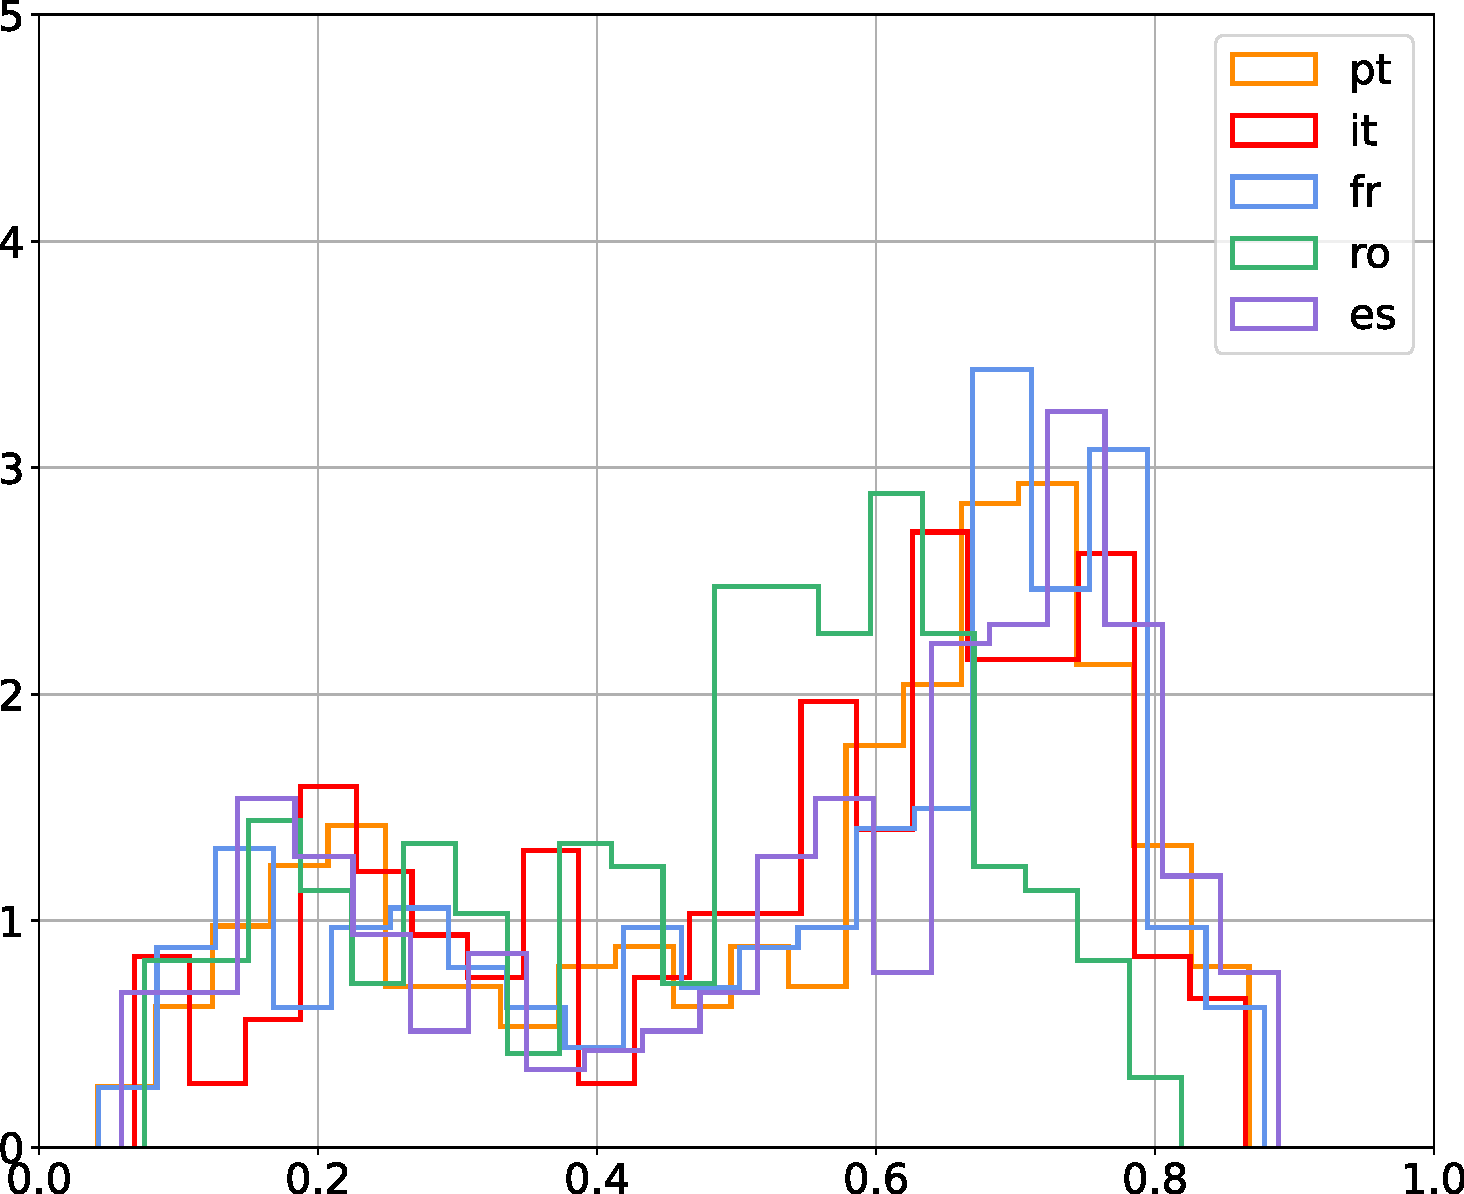
\includegraphics[width=\linewidth]{figures/UBAN_histogram_distances_en_all_contour_complete}
        \caption{English vs all}
    \end{subfigure}
    
    \caption{\label{fig:exp1}Distributions of cross-lingual similarity scores between cognates.}
\end{figure*}

Another interesting observation relates to the distributions of scores for each language pair, shown in the histograms in Figure~\ref{fig:exp1}. While similarity scores between cognates among Romance languages usually follow a normal distribution (or another unimodal, more skewed distribution), the distributions of scores for Romance languages with English seem to follow a bimodal distribution, pointing to a different semantic evolution for words in English that share a common etymology with a word in a Romance language. One possible explanation is that the set of cognates between English and Romance languages (which are pairs of languages that are more distantly related) consist of two distinct groups: words that were borrowed directly from the Romance language to English (which should have more meaning in common), and words that had a more complicated etymological trail between languages (and for which meaning might have diverged more, leading to lower similarity scores). 

\citet{cognatesuban:beinborn2019semantic} have shown that when comparing a list of core words between languages in aligned embedding spaces, the average similarities differ between different language pairs, due to artifacts of the aligned embedding space itself, which is a possible confounding factor for our results. Translation pairs in two languages tend to be closer in the embedding space for more similar languages. Thus, any observed difference between average cognate similarity scores across language pairs could also be explained by the underlying properties of the embedding spaces, at the level of the overall vocabulary, and not an effect of semantic divergence between cognate pairs specifically.

We further attempt to test the validity of our hypothesis that the observed cognate-based similarities between languages are, at least to some degree, specific to cognates, and thus can be interpreted as reflecting the process of cognate divergence. We compare the obtained similarities based on cognate pairs with baseline similarities between manually built translation pairs, using the seed dictionaries in \citet{cognatesuban:conneau2017word}, which contain approximately 100,000 word pairs for each language pair (between 87,000 and 113,00 across all included language pairs). We compute these for the language pairs where seed dictionaries were available (so excluding Romanian and Latin). A difference between similarities based on translation pairs and similarities based on cognate pairs would confirm that cognate divergence does contribute the observed effect (which is not simply due to embedding space alignment). The baseline used here differs from the one reported in Section \ref{section:introduction} where we sample word similarities across the entire embedding space randomly, as opposed to focusing on translation pairs.

\begin{figure}
    \centering
    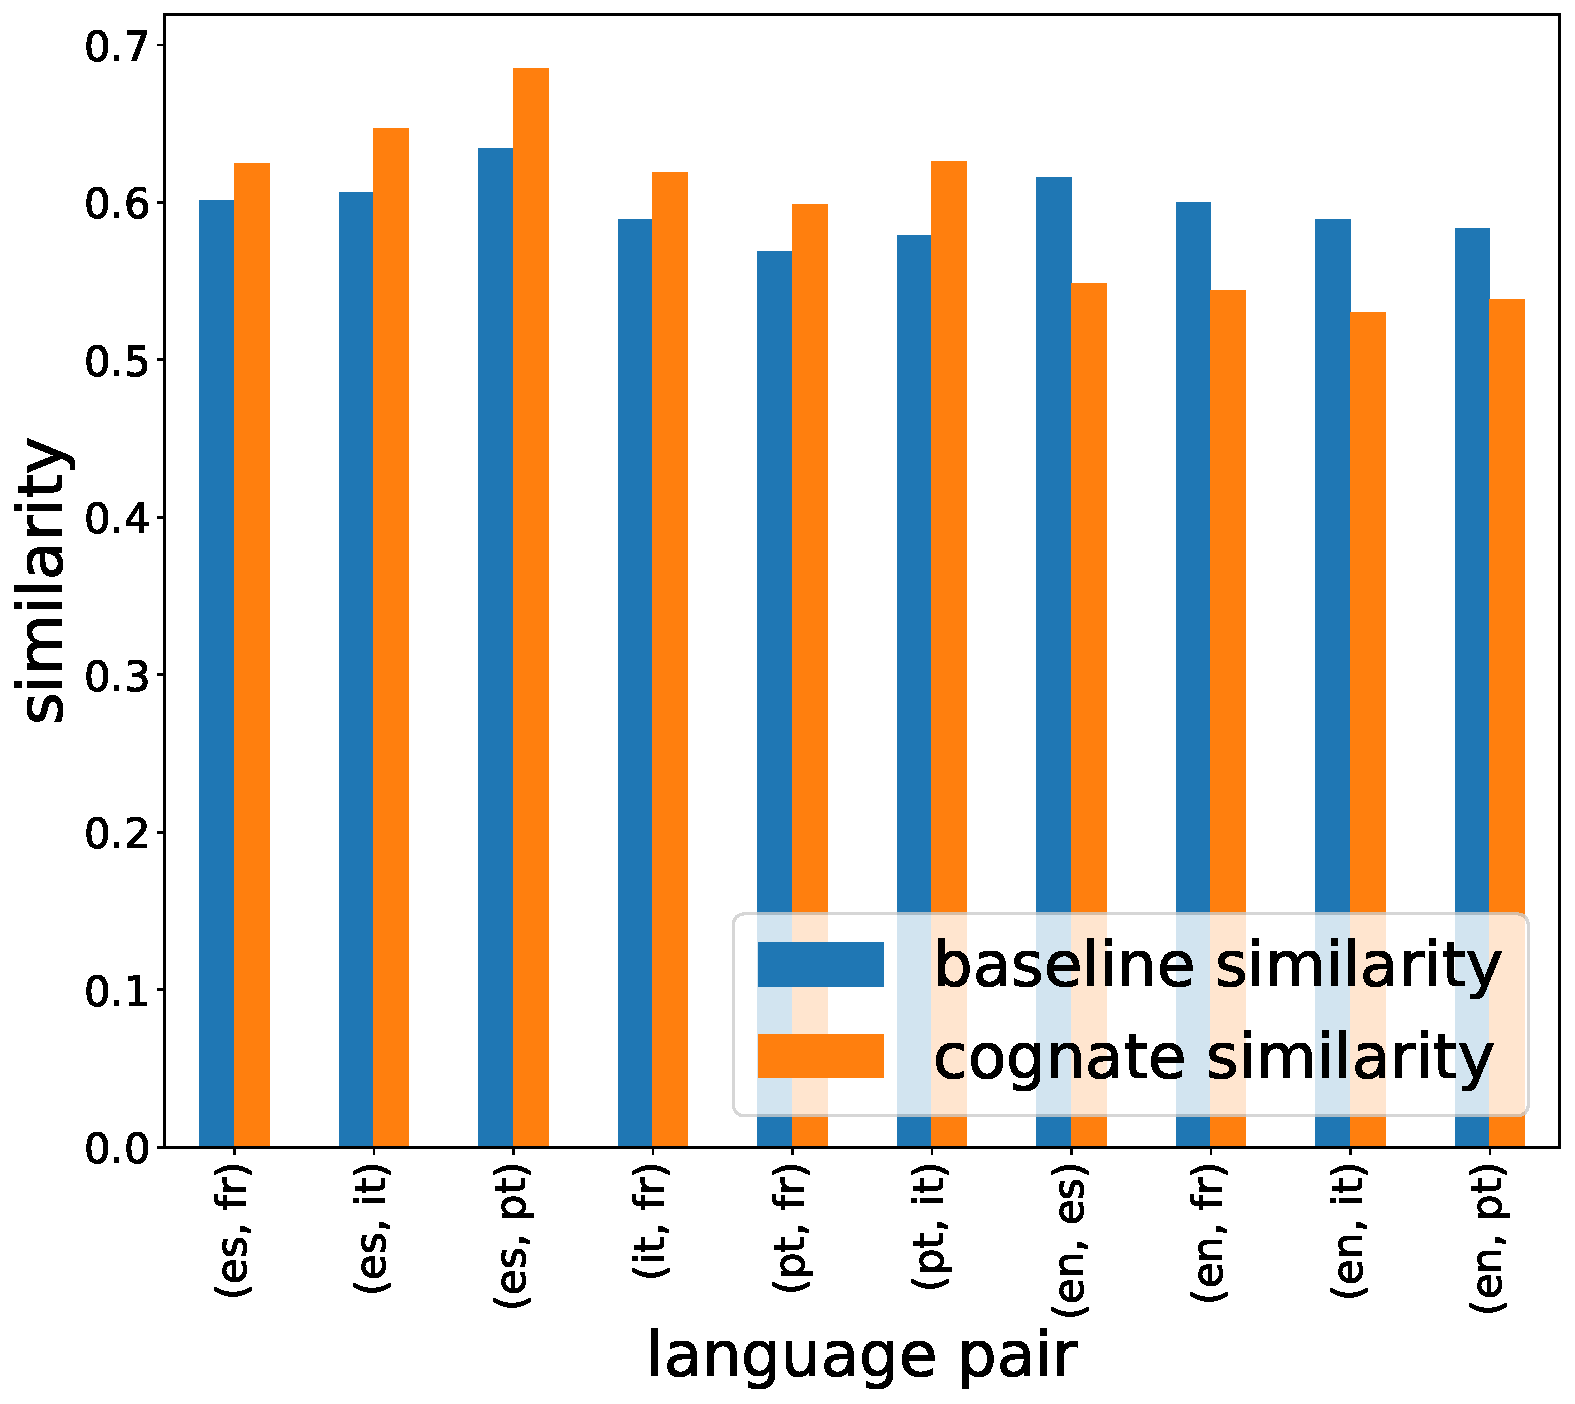
\includegraphics[width=0.5\linewidth]{figures/UBAN_baseline_vs_cognates_similarities_bar.pdf}
    \caption{Comparison of language similarity scores based on baseline dictionaries and on cognate pairs.}
    \label{fig:baseline_vs_cognates}
\end{figure}

Table~\ref{table:seed_similarity_en} shows average similarities for seed translation pairs, and Figure \ref{fig:baseline_vs_cognates} illustrates direct comparisons of average similarities for baseline terms and for cognate pairs. Here we notice a pattern of higher cognate-based similarity for Romance languages compared to the baseline, and lower cognate similarities for pairs involving English.

Beyond these differences, we notice however that translation similarities are not uniform across language pairs either, showing a similar pattern to cognate similarities. This would entail that the observed effect in differences between language pairs, and hypothesized higher similarity between closer languages (such as Spanish and Portuguese), is at least partly due to imperfect embeddings alignment noise. To compare the contribution of embedding alignment noise to that of cognate divergence, we compute the Spearman correlation between the cognate-based distances and the translation-based distances for every language pair (for a total of $10$ language pairs), in order to verify whether the relative order of language pairs in terms of average similarities is different in cognates and seed translations, and we obtain a correlation of $0.36$ ($p$-value $0.32$). 
We conclude that there is a noticeable effect related to cognate divergence, but that alignment noise should be kept in mind when interpreting the results, and further research based on more refined alignment algorithms or a different class of methods for measuring cross-lingual semantic distance would be useful for a more conclusive result. We leave for future work a similar analysis for the missing language pairs, including Romanian and Latin, with the possible inclusion of additional baseline word pairs, such as the ones used in \citet{cognatesuban:beinborn2019semantic}.

\begin{table}[!ht]
\begin{center}
\begin{tabular}{l l l l l l l}
\lsptoprule
& Fr & It & Pt &  En \\
\midrule

Es & 0.60 & 0.60  & 0.63 &  0.61   \\
Fr & & 0.58 & 0.56 &   0.59   \\
It & & & 0.57 &   0.58   \\
Pt & & & &   0.58   \\
\lspbottomrule

\end{tabular}
\end{center}
\caption{\label{table:seed_similarity_en}Average cross-lingual similarity between seed translation pairs.}
\end{table}

\section{Detection and correction of false friends}\largerpage
\label{section:false-friends}

In this section, we propose using a fully automatic and unsupervised algorithm in order to detect false friends, and we generate a lexicon of false friends, along with falseness scores for each pair, for every language pair among six considered languages (five Romance languages and English). Our method is based on the false friend detection algorithm relying on cross-lingual word embeddings introduced by \citet{cognatesuban:uban2019cognates}, to which we add a more extensive evaluation of the resulted false friends pairs, including the extended list of over 3,000 cognate sets (instead of the smaller 305 words list evaluated in the previous study) and additionally include an evaluation and analysis of the falseness measure. We publish freely the resulting database comprising of false friend pairs for each pair of considered languages, and the falseness score for each pair.

Our chosen method of leveraging word embeddings extends naturally to another application related to this task which, to our knowledge, has not been explored so far in research: false friend correction. We propose a straightforward method for solving this task of automatically suggesting a replacement when a false friend is incorrectly used in a translation. Solving this problem could result in a tool especially useful for language learners to help them use language correctly.

\subsection{Algorithm}\largerpage

In the following subsection, we describe the algorithm used for detecting false friends automatically, in an unsupervised manner, based on a seed set of cognate sets, as well as a method for correcting false friends.
Using the same principles as in the previous experiment, we can use embedding spaces and semantic distances between cognates in order to detect pairs of false friends, which are simply defined as pairs of cognates which do not share the same meaning, or which are not semantically similar \textit{enough}.

False friends can be identified as pairs of cognates with high semantic distance. More specifically, we consider a pair of cognates to be a false friend pair if in the shared semantic space, there exists a word in the second language which is semantically closer to the original word than its cognate pair in that language (in other words, the cognate is not the optimal translation). The arithmetic difference between the semantic distance between these words and the semantic distance between the cognates will be used as a measure of the \textit{falseness} of the false friend. 

The algorithm has the additional ability to provide suggestions for correcting false friends: the nearest neighbor (in the second language) to the first cognate will be the suggested ``correction'', which should correspond to the correct translation of the cognate. This solution is based on the principle used in \textsc{bilingual lexicon induction} (BLI), which is the task of automatically discovering words with the same meaning across languages \citep{cognatesuban:mikolov2013exploiting,cognatesuban:heyman2017bilingual}: our algorithm can be seen as an application of BLI. In previous literature, multilingual embedding spaces have been used for BLI \citep{cognatesuban:vulic-moens-2015-bilingual}; we propose they can be useful in the context of false friends and language learning. The approach is described in detail in Algorithm~\ref{Detection and correction of false friends}.


\begin{algorithm}
\caption{Detection and correction of false friends}
\label{Detection and correction of false friends}
\SetAlgoLined
Given the cognate pair $(c_1, c_2)$ where $c_1$ is a word in $lang_1$ and $c_2$ is a word in $lang_2$:\\
Find the nearest neighbor of $c_1$ in $lang_2$ as the word $w_2$ in $lang_2$ such that for any $w_i$ in $lang_2$, $distance(c_1, w_2) < distance(c_1, w_i)$\\
\If{$w_2 \neq c_2$}{
	$(c_1, c_2)$ is a pair of false friends\\
	Degree of falseness $= distance(c_1, w_2) - distance(c_1, c_2)$\\
\Return $w_2$ as potential correction
}

\end{algorithm}



  \begin{table}
\begin{tabular}{l l l l}
\lsptoprule
Cognate & False friend & Correction & Falseness \\\midrule
long (Fr) & luengo (Es) & largo & 0.50 \\
face (Fr) & faz (Es)  & cara & 0.39 \\
change(Fr)  & caer (Es) & cambia & 0.46 \\
\midrule
stânga (Ro) & stanco (It) & destra & 0.52 \\
tânăr (Ro) & tenero (It) & giovane & 0.41 \\
inimă (Ro) & anima (It) & cuore & 0.13 \\
amic (Ro) & amico (It) & amichetto & 0.04 \\
\lspbottomrule

\end{tabular}

\caption{\label{table:ff_examples2}Extracted false friends and falseness.}
\end{table}


We select a few results of the algorithm to show in Table \ref{table:ff_examples2}, containing examples of extracted false friends, along with the suggested correction and the computed degree of falseness.
The table shows some examples of the algorithm correctly identifying and correcting false friends pairs -- such as the Romanian-Italian pairs \textit{tânăr} `young'\slash\textit{tenero} `tender', with the Italian correction \textit{giovane} `young', or \textit{inimă} `heart'\slash\textit{anima} `soul', corrected to \textit{cuore} `heart'. The falseness scores also reflect the degree of semantic drift between the false friends, with the \textit{tânăr}\slash\textit{tenero} pair being more dissimilar than \textit{inimă}\slash\textit{anima}. The \textit{amic}\slash\textit{amico}\slash\textit{amichetto} set, which refers to different degrees of friendship, is awarded the lowest falseness score.
It is valuable to note the algorithm also selects word pairs which can technically be considered true cognates (\textit{long}\slash\textit{luengo} -- meaning `long', but are not used as such in current speech: \textit{largo} is more frequently used than \textit{luengo}.\largerpage{} This is to be expected since the algorithm is based on word \textit{usage} in language (since this is the basis of the embedding training algorithm). 
We also illustrate an example where the algorithm makes a mistake: in the case of \textit{stânga} `left'\slash\textit{stanco} `tired', the algorithm rightly identifies this as a false friends pair, but provides an erroneous correction: \textit{destra} is the Italian word for `right', not `left'. This error can also be traced back to the nature of semantic similarity as captured by word embeddings: related but not equivalent words (and sometimes even antonyms) can have similar embedding vectors due to their similar occurrence patterns in corpora.

\subsection{Building a false friends dataset}

We use the algorithm described in the previous subsection to build a database of false friends pairs for each language pair among the six considered languages, which we make freely available.\footnote{\url{https://github.com/ananana/false\_friends_resource}}
False friends for Romance languages are extracted from the original 3,218 cognate sets, resulting in 500 to 1,200 pairs of detected false friends for each language pair. For English, the original cognate resource contains a smaller set of only 305 cognate sets, which results in smaller false friends lists for language pairs involving English.
Table \ref{tab:ff_db} shows the number of false friends pairs generated for each language pair, and included in the published resource.

\begin{table}[!h]
    \centering
    \begin{tabular}{l r p{0.05\textwidth} l r}
         \lsptoprule
         Languages & FF Pairs & & Languages & FF Pairs \\
         \midrule
            Es--It & 739 &   & It--Es & 727 \\
            Es--Pt & 490 &   & Pt--Es & 502 \\
            Fr--It & 921 &   & It--Fr & 925 \\
            Fr--Es & 886 &   & Es--Fr & 905 \\
            Fr--Pt & 1,023 & & Pt--Fr & 1,060 \\
            It--Pt & 795 &   & Pt--It & 848 \\
            Ro--Fr & 1,258 & & Fr--Ro & 1,596 \\
            Ro--It & 1,286 & & It--Ro & 1,654 \\
            Ro--Es & 1,229 & & Es--Ro & 1,647 \\
            Ro--Pt & 1,227 & & Pt--Ro & 1,640 \\
            En--Pt & 148 &   & Pt--En & 137 \\
            En--Es & 158 &   & Es--En & 136 \\
            En--It & 153 &   & It--En & 139 \\
            En--Fr & 150 &   & Fr--En & 133 \\
            En--Ro & 205 &   & Ro--En & 161 \\
            
         \lspbottomrule
    \end{tabular}
    \caption{Number of datapoints in false friends database.}
    \label{tab:ff_db}
\end{table}


\subsection{Evaluation}

In order to evaluate the quality of the false friends dataset generated with our algorithm, we first test its accuracy against a multilingual dictionary. For this study, we choose to use Open Multilingual WordNet \citep{cognatesuban:miller1998wordnet,cognatesuban:bond2013linking}. WordNet is a semantic network organized in synsets which represent concepts, where each word is part of as many synsets as concepts it designates. Two words with common etymology are considered true cognates if they belong to the same WordNet synset (are synonyms), and false friends if they are found in WordNet, but not as synonyms. Cognates not found in any WordNet synset are not considered. Using this standard, the obtained measured accuracy is between 73\% and 81\%, depending on the considered language pair. Table \ref{table:results_ff} presents a breakdown of the obtained performance per considered language pair. Romanian is the only language missing from the evaluation since it is not represented in multilingual WordNet. Since English cognates are only available for a subset of the cognates list, our evaluation results for Romance languages may be more robust.

\vfill
\begin{table}[H]
\begin{tabular}{lccc}
\lsptoprule
& Accuracy & Precision & Recall\\
\midrule
Es--It & 73.69 & 43.27 & 38.06 \\
It--Es & 73.58 & 43,12 & 37.73 \\
Es--Pt & 79.09 & 36.05 & 26.49 \\
Pt--Es & 78.65 & 32.32 & 24.35 \\
Fr--It & 74.43 & 33.39 & 57.40 \\
It--Fr & 74.77 & 34.32 & 58.68 \\
Fr--Es & 76.25 & 42.02 & 51.94 \\
Es--Fr & 75.13 & 40.27 & 51.78 \\
It--Pt & 74.58 & 33.20 & 44.73 \\
Pt--It & 73.61 & 31.69 & 49.31 \\
\midrule
En--Pt & 77.25 & 59.81 & 86.48 \\
Pt--En & 79.82 & 64.70 & 85.71 \\
En--Es & 76.58 & 63.88 & 88.46 \\
Es--En & 80.48 & 71.57 & 83.95 \\
En--It & 77.40 & 61.73 & 87.65 \\
It--En & 74.89 & 61.90 & 76.47 \\
En--Fr & 77.09 & 57.89 & 94.28 \\
Fr--En & 81.05 & 66.32 & 86.66 \\
\lspbottomrule
\end{tabular}
\caption{\label{table:results_ff}Performance for all language pairs using WordNet as the gold standard.}
\end{table}
\vfill\pagebreak




In a second experiment, we measure the accuracy of false friend detection on a manually curated list of false friends and true cognates in Spanish and Portuguese, used in a previous study \citep{cognatesuban:castro2018high}, and introduced by \citet{cognatesuban:torres2011using}. This resource is composed of 710 Spanish-Portuguese word pairs: 338 true cognates and 372 false friends. We also compare our results to the ones reported in this study, which uses a method similar to ours (using a simple classifier that takes embedding similarities as features to identify false friends) and shows improvements over results in previous research. The results are shown in Table \ref{table:exp1}. We also compute the same metrics using a falseness threshold as a lower bound to decide whether two words are false friends, and observe a trade-off between recall and precision when using a threshold. The following subsection discusses the use of falseness thresholds in more detail.

In this second experiment, WordNet is used as a baseline algorithm for false friend identification instead of a gold standard. Its relatively poor results (reported in Table~\ref{table:results_ff}), in comparison with the automatic methods, may stem from its coverage, which is lower than for corpus-based methods. \citet{cognatesuban:castro2018high} show that only 55\% of the word pairs in the evaluation set used here are found in WordNet synsets. This shows that using WordNet as an evaluation standard has its limits, and that corpus-based methods for evaluating cross-lingual semantic similarity, such as the one we propose, have an advantage over dictionary-based methods.

\begin{table}
\begin{tabular}{lccc}

\lsptoprule
& Accuracy & Precision & Recall\\
\midrule

Our method ($\text{ft}=0$) & 81.81 & 78.69 & 80.80 \\
Our method ($\text{ft}=0.1$) & 82.62 & 92.37 & 66.06 \\
\midrule
\citet{cognatesuban:castro2018high} & 77.28 & --  & -- \\
\citet{cognatesuban:torres2011using} & 76.37 & -- & -- \\
WN Baseline & 69.57 & 85.82 & 54.50 \\
\lspbottomrule
\end{tabular}
\caption{\label{table:exp1}Performance for Spanish-Portuguese using curated false friends test set, compared to previous attempts.}
\end{table}

\subsubsection{Falseness as a spectrum}
The measure of falseness that we provide for every detected pair of false friends can be useful not only for a better understanding of the linguistic phenomenon behind the semantic divergence of the cognates, but also for a more flexible integration with downstream applications. When using our resource of false friends, a custom threshold of falseness could be set for filtering out false friends in a more coarse or fine-grained way, depending on the needs of the application: by selecting as false friends only pairs with falseness above a specific (non-zero) threshold. For example, for applications where capturing subtle changes in meaning is important, maintaining a low threshold of falseness is useful. On the other hand, when the goal is to only identify false friends which have entirely different meanings, choosing a high threshold may be sufficient. It might also ensure a lower rate of false positives by filtering out the delicate cases of cognates which lie at the boundary between true and deceptive cognates.\largerpage

\begin{figure}
    \centering
    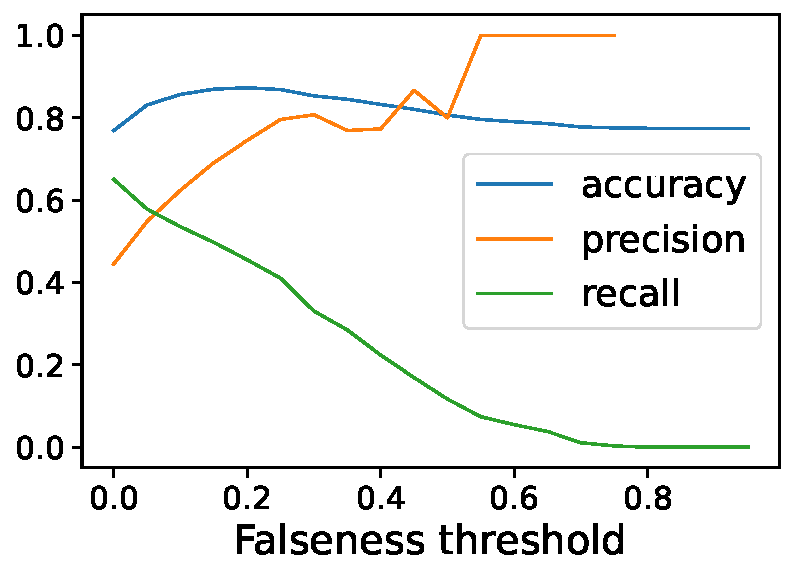
\includegraphics[width=0.66\textwidth]{figures/UBAN_falseness_vs_accuracy.pdf}
    \caption{Performance with falseness threshold.}
    \label{fig:false_vs_acc}
\end{figure}

We perform an analysis of the effect of varying the threshold applied to the falseness score in order to discriminate between true cognates and false friends, by re-evaluating the generated false friends against WordNet using different threshold values (as opposed to the simple evaluation in the previous section, where no threshold was set, which is equivalent to using a falseness threshold of 0). In this way, we are able to discover the optimal falseness threshold to use in order to maximize performance relative to the WordNet standard. We choose the threshold which leads to maximum average accuracy across all language pairs on a separate training set of 80\% of the word pairs. The rest of 20\% of the word pairs are used to evaluate the method, now employing a falseness threshold set to the optimal value according to the training phase. The optimal falseness threshold $\textit{ft}\star$ is found to be 0.2, and the average overall accuracy with this threshold is 85.85\%. Table~\ref{tab:overall_acc} shows the difference in accuracy when using the optimal threshold, and Figure~\ref{fig:false_vs_acc} illustrates the variation of accuracy, precision and recall (on average for all language pairs) when varying the threshold between 0 and 1.

\begin{equation}
\textit{ft}\star = \text{argmax}_{\textit{ft} \in (0,1)}\frac{1}{|\text{LP}|}\sum_{l_1,l_2 \in \text{LP}}{\text{Acc}(\textit{ft},l_1,l_2)}
\end{equation}
where \textit{ft} is a falseness threshold and LP is the set of all language pairs:
\begin{equation}
    \text{LP} = \{(l_1,l_2) | l_1, l_2 \in \{\text{Ro, Es, Pt, Fr, It, En}\}\}
\end{equation}

The fact that in WordNet the optimal falseness threshold is positive (non-zero) suggests that many of the pairs with very low falseness make up for most of false positives (actual true cognates) and are responsible for a drop in accuracy (as they are probably identified as false friends by the algorithm not necessarily because they are actually different in meaning, but rather because of artifacts of the embedding space).

\begin{table}[!h]
    \centering
    \begin{tabular}{c c c}
\lsptoprule
Falseness threshold & 0 (None) & 0.2 (optimal) \\
\midrule
Accuracy & 80.57 & 85.85 \\
\lspbottomrule
    \end{tabular}
    \caption{Best overall accuracy of our method.}
    \label{tab:overall_acc}
\end{table}

We then perform the same experiment, but this time evaluate using the curated cognate sets in Spanish-Portuguese. In this case, the optimal threshold is found to be 0.1, and the threshold of 0.2 found in the previous experiment leads to worse results than not using a threshold at all. In order to confirm that the difference stems from the the different definition of cross-lingual synonymy in the two datasets and is not specific to just the language pair, we compute the optimal falseness threshold relative to WordNet specifically for Spanish-Portuguese and find an optimal value of 0.3. One explanation for the different optimal thresholds on the two reference datasets may be that they cover different parts of the vocabulary, as confirmed by the previously reported low coverage of WordNet on the Spanish-Portuguese test set. The difference between the optimal threshold values for the two different gold standards may also suggest that the two resources were built based on different assumptions about meaning equivalence, and confirms that the availability of the falseness measure can be useful for tuning the false friend detection algorithm to the specific task and standards of the particular application.

\subsubsection{Error analysis and discussion}

As suggested in the previous subsection, a significant source of error relative to the WordNet standard are low-falseness pairs of detected false friends.
Figures~\ref{false_hist1} and~\ref{false_hist2} show the distribution of falseness scores across all word pairs in all languages. We separately show the distribution of false friends extracted with our method that were evaluated as actual false friends using WordNet, and the pairs of extracted false friends that are actually true cognates according to WordNet. The much lower falseness values for word pairs in the second category (false positives in the evaluation using WordNet) suggest that many of the false positives produced by the algorithm fall in the range of word pairs with very subtle differences in meaning. These might stem from imperfections in the embedding space or from the too strong assumption that the closest word in the multilingual embedding space is the correct translation. Some of the examples in Table~\ref{table:ff_examples2} illustrate these types of error; such is the case of the previously discussed pair \textit{stânga}\slash\textit{stanco}, with the mistaken correction \textit{destra}. More subtle inaccuracies can consist, for example, of mismatched parts of speech, such as the case of \textit{change} (noun)\slash\textit{caer} (infinitive verb)\slash\textit{cambia} (indicative verb).

\begin{figure}
  \captionsetup{margin=.05\linewidth}
    \begin{floatrow}
        \ffigbox{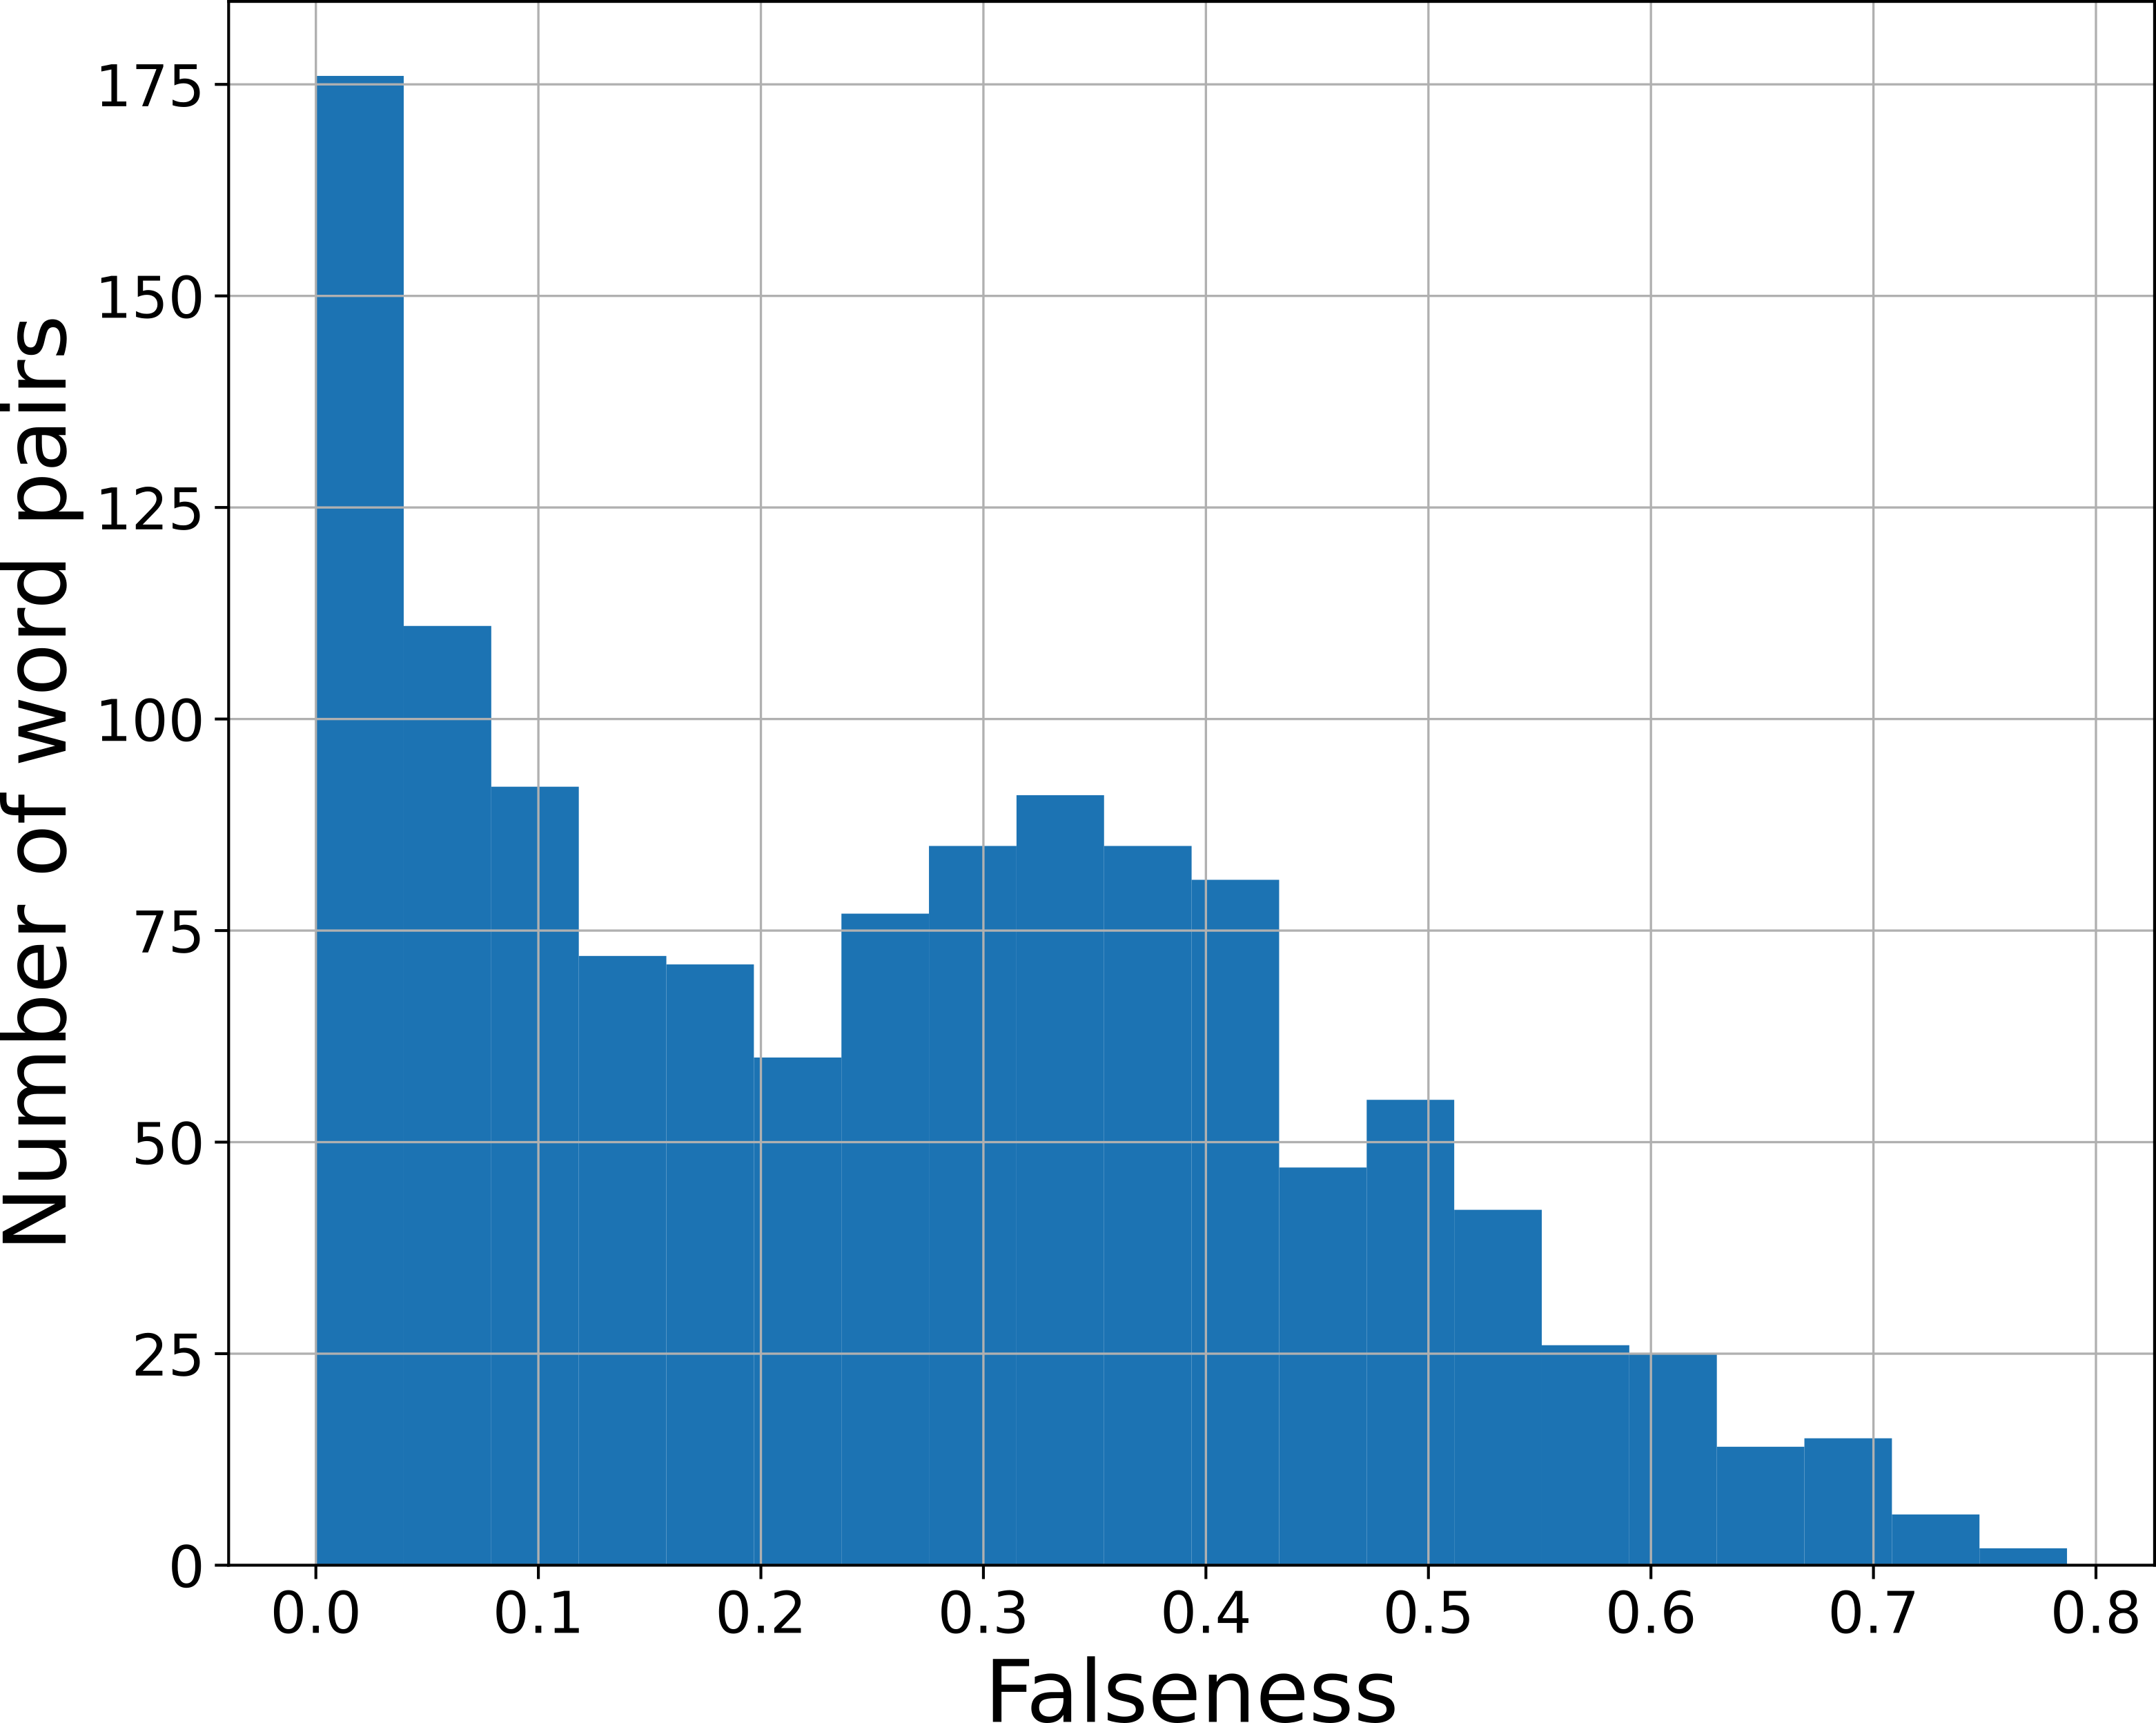
\includegraphics[width=.5\textwidth]{figures/UBAN_falseness_ff_hist.png}}
                {\caption{Falseness in correctly detected false friends.\label{false_hist1}}}
        \ffigbox{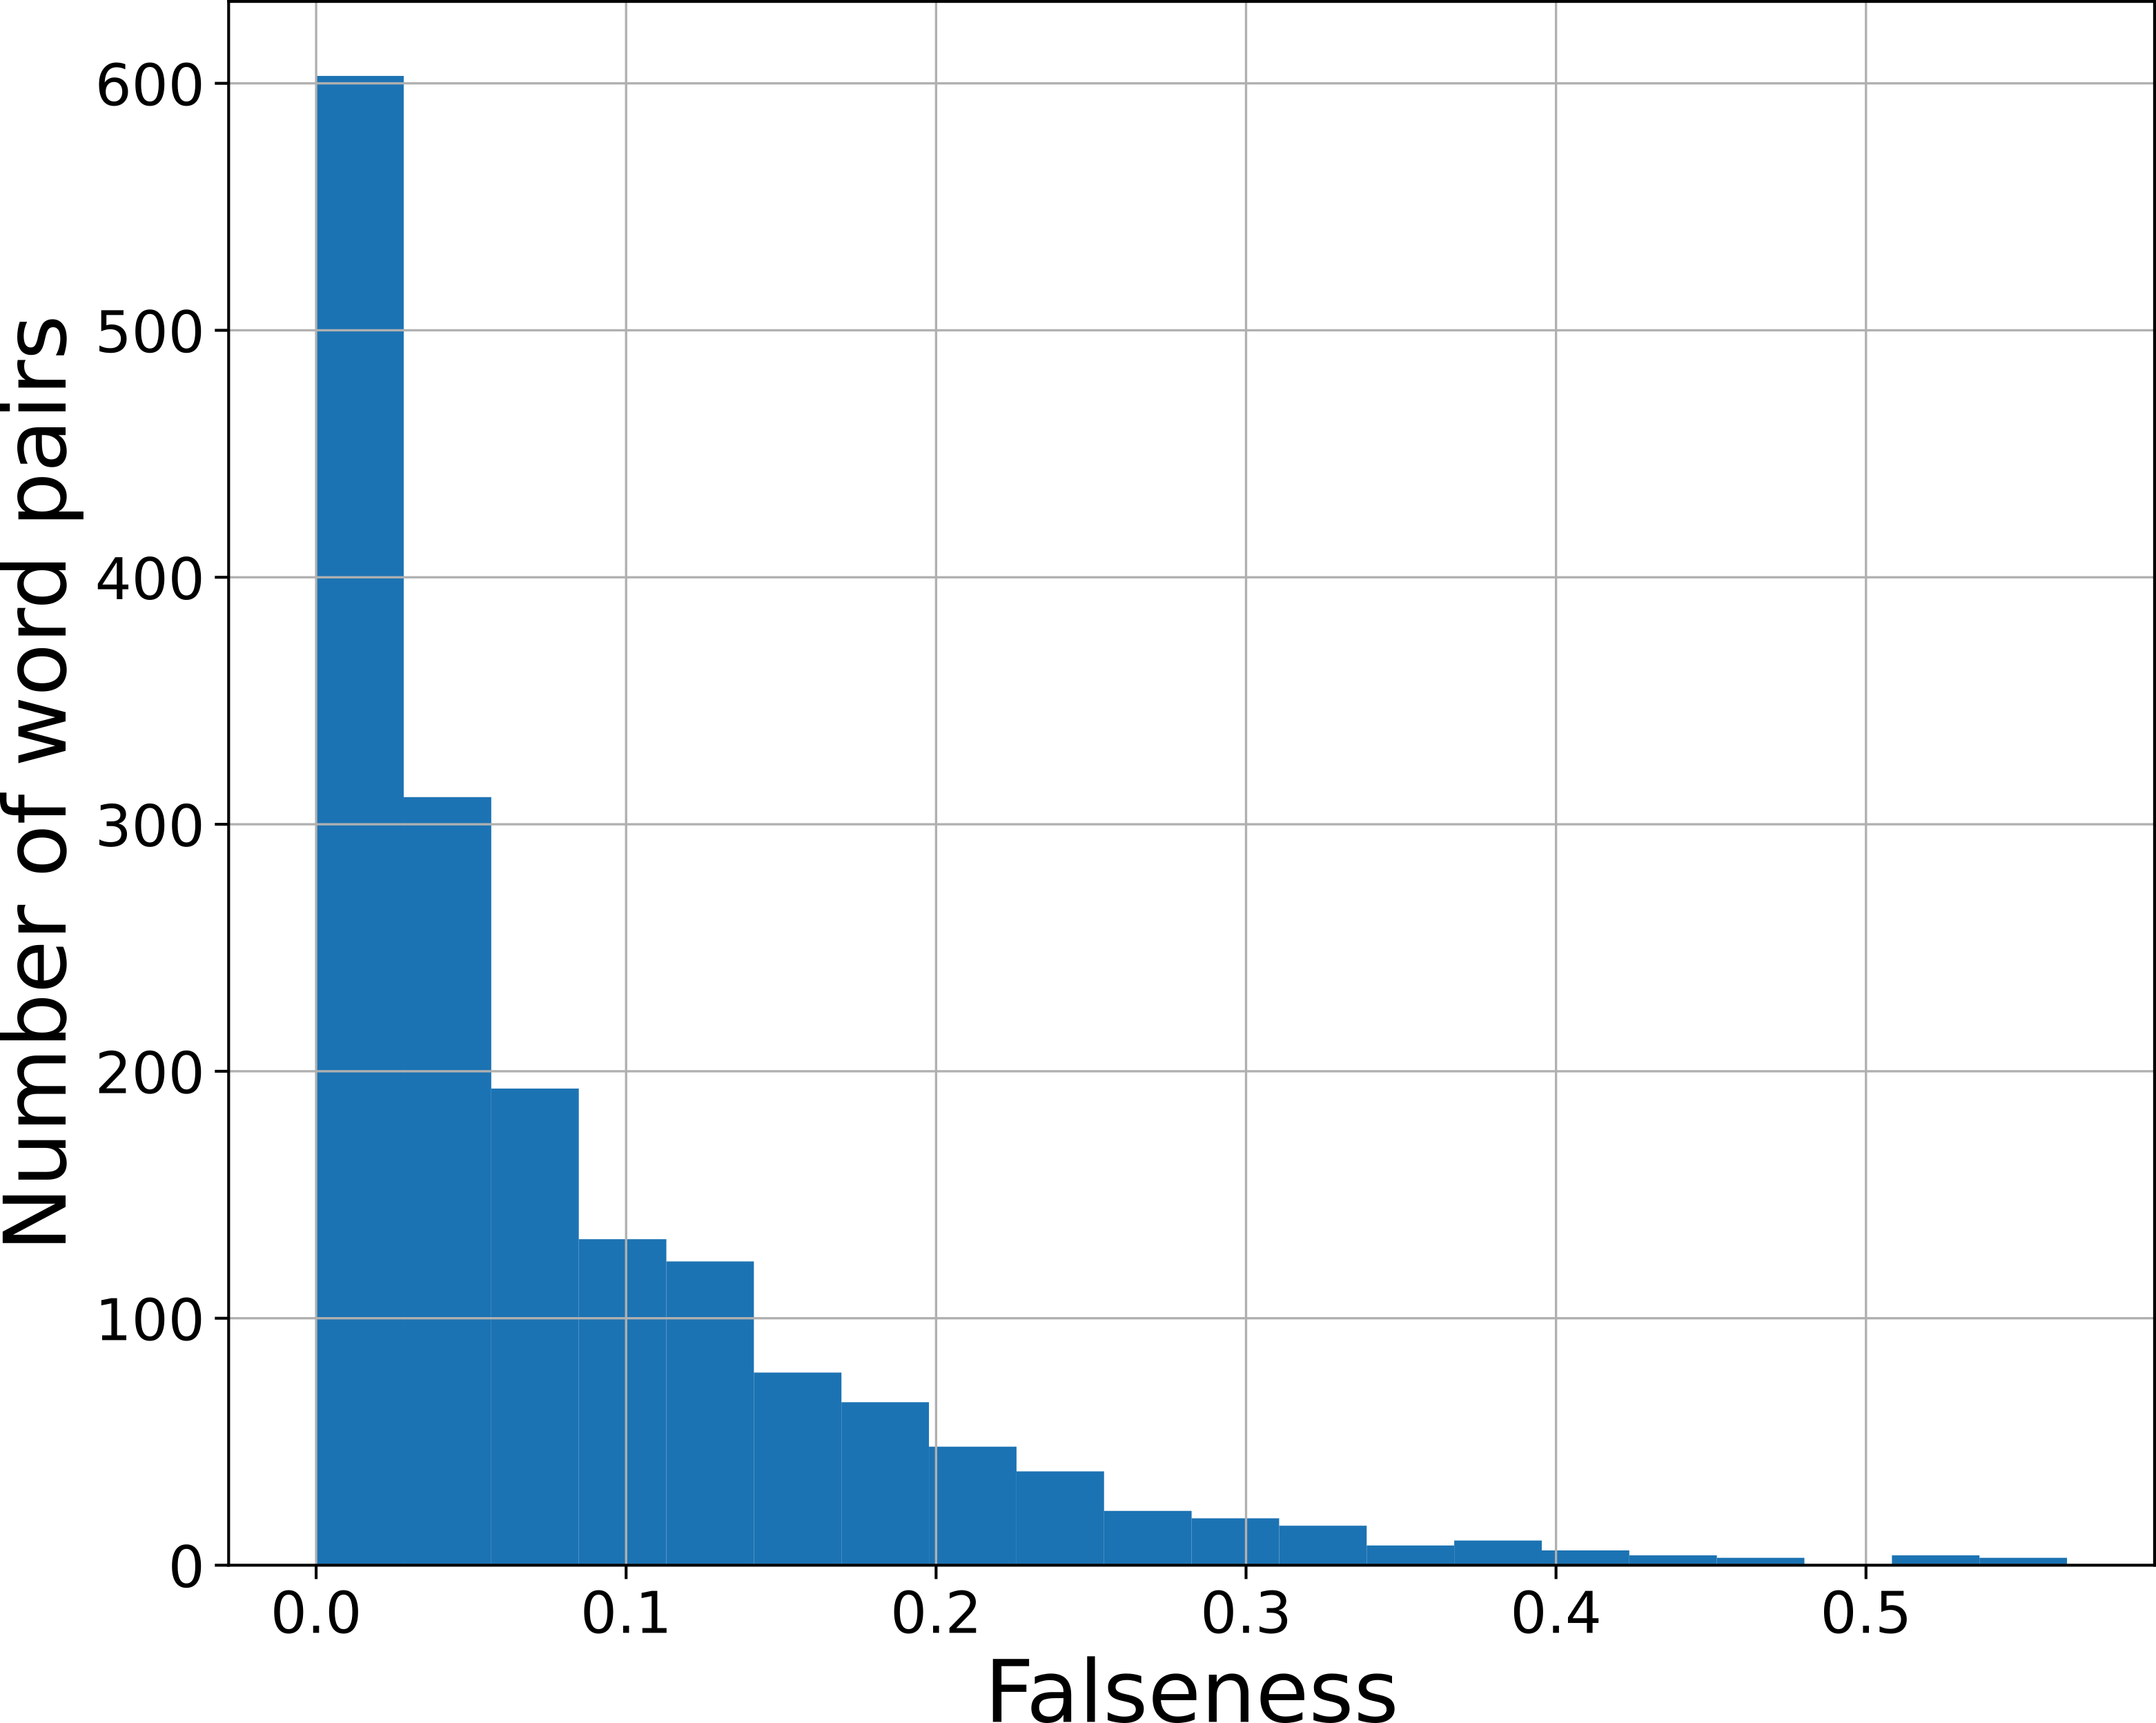
\includegraphics[width=.5\textwidth]{figures/UBAN_falseness_notff_hist.png}}
                {\caption{Falseness in incorrectly detected false friends.\label{false_hist2}}}
    \end{floatrow}
\end{figure}

We argue that including the falseness score in our published lexicon of false friends can be useful precisely to remedy this issue when needed, by setting a higher threshold on the falseness score. On the other hand, it is possible that in some cases, the low-falseness word pairs classified as false positives according to WordNet could even be considered actual false friends (rather than errors of classification) by a standard of meaning equivalence that is more strict than the one used in WordNet's synsets, again confirming the value of modelling falseness as a spectrum.

A second source of errors is found in the original cognates data source that we use to discriminate into true and false cognates. Since it is also an automatically built resource, some of the word pairs are falsely labelled as cognates, and may further perpetuate into false positives in our algorithm.

\section{Laws of cross-lingual semantic change}
\label{section:laws-of-semantic-change}


We use the measure of falseness of a deceptive cognate pair to quantify the semantic shift between the meanings of a word derived from the same etymon in different languages. We further propose analyzing how the properties of frequency and polysemy of a word relate to semantic shift, and, analogously to what \citet{hamilton-etal-2016-diachronic} do for monolingual semantic change, we aim to move towards uncovering statistical laws of semantic change across languages.


In the next subsection, we first define a measure of the frequency of a word, as well as a measure of its polysemy. Further, we try to correlate these measures of frequency and polysemy with the falseness measure defined in the previous subsections. Finally, we find mathematical equations that best describe the relationship between frequency and polysemy of words in a cognate pair on one hand, and the falseness degree of the pair on the other hand, according to our dataset. As a preliminary step, we discard all cognate pairs that, according to the false friend detection algorithm, are true cognates, and focus only on the deceptive cognates, for which falseness scores are non-zero. On average across all language pairs, 37\% of the cognate pairs in our dataset are found as deceptive cognates. Moreover, we validate these results using multilingual WordNet, and further select only pairs which are confirmed to be deceptive cognates as such: two cognates are considered to be true cognates if they are synonyms according to WordNet, and are considered to be deceptive cognates otherwise. It should be noted that having to use WordNet limits us to languages for which WordNet is available (which excludes Romanian, for which we consider all words in the cognate set instead).

Through characterizing the relationship between frequency and polysemy on the one hand, and semantic change (as measured by falseness in our case) on the other hand, we aim to discover statistical laws that describe how semantic change of words relates to other properties of the words. Similar attempts at formulating laws of semantic change have been made in previous studies in monolingual diachronic settings, with the notable example of \citet{hamilton-etal-2016-diachronic}, who find polynomial relationships between the same word properties (frequency, polysemy) and the degree of semantic change over time. Nevertheless, an important difference is that while the authors of the monolingual study correlate the rate of the shift of meaning for a word to its frequency and polysemy \textit{prior} to the change in meaning, our method looks at the magnitude of the meaning shift in comparison with properties of words \textit{after} the meaning shift has already occurred, presumably from the original meaning of the proto-word they derive from to their current meanings in their respective languages.

\subsection{Word frequency and semantic divergence}

For measuring \textit{frequency}, we use the multilingual Wordfreq Python library \citep{cognatesuban:robyn_speer_2018_1443582}, which estimates word frequency based on multiple corpora (such as Wikipedia and Twitter). 
For most of the languages we consider, we are able to extract frequency scores for the majority of words in our cognate sets, with a coverage of at least 92\% of the words in our cognate set for every language considered, except for Romanian, which has a poorer coverage of only 60\%.


For each pair of languages in a cognate set, we compute the Spearman correlation between the average of the frequencies of the words in the cognate pair and the falseness of the deceptive cognate. Since frequency and polysemy are correlated, we need to control for polysemy in order to observe the marginal effect of frequency on semantic divergence. To this effect, we compute partial correlations, using polysemy as a covariate variable. Similarly, when computing correlations for polysemy, we set frequency as a covariate.

The results showing the correlations for each language pair are reported in Table \ref{tab:freq-corr}. The values show a positive correlation, with values up to $0.33$ (for Italian-French), suggesting that the frequency of a cognate word is related to the degree of semantic change it suffered, independently from polysemy.

We further try to understand the nature of the relationship between frequency and falseness. Previous studies \citep{hamilton-etal-2016-diachronic} showed that prior frequency relates to subsequent semantic shift according to a power law. In our setup, we study the effect of previous semantic shift on the frequency of words. We model this relation by comparing the logarithm of the (average) frequency for a word pair with the falseness degree of the pair. To obtain the log-frequency, we use the Zipf frequencies provided by the Wordfreq library, which are computed as the base-10 logarithm of the number of times it appears per billion words. We first plot the log-frequency against the falseness degree, shown for Spanish-Portuguese in Figure~\ref{fig:scatter2}. 

\begin{table}[p]
    \begin{tabular}{l  *{6}{S[table-format=-1.3]} }
    \lsptoprule
        &  {Es} & {Pt} & {It} & {Fr} & {Ro} & {En} \\ \midrule
        Es &  & 0.219 & 0.11 & 0.201 & 0.007 & 0.08 \\
        Pt & 0.212 &  & 0.048 & 0.161 & 0.148 & 0.2 \\
        It & 0.089 & -0.007 &  & 0.334 & 0.129 & 0.083 \\
        Fr & 0.188 & 0.117 & 0.323 &  & 0.194 & 0.3 \\
        Ro & 0.062 & 0.148 & 0.147 & 0.271 &  & 0.229 \\
        En & 0.161 & 0.242 & 0.083 & 0.315 & 0.163 &  \\
        \lspbottomrule
    \end{tabular}
    \caption{Correlations of frequency with falseness, controlling for polysemy.\label{tab:freq-corr}}
\end{table}

\begin{figure}[p]
    \begin{subfigure}{0.5\textwidth}\centering
    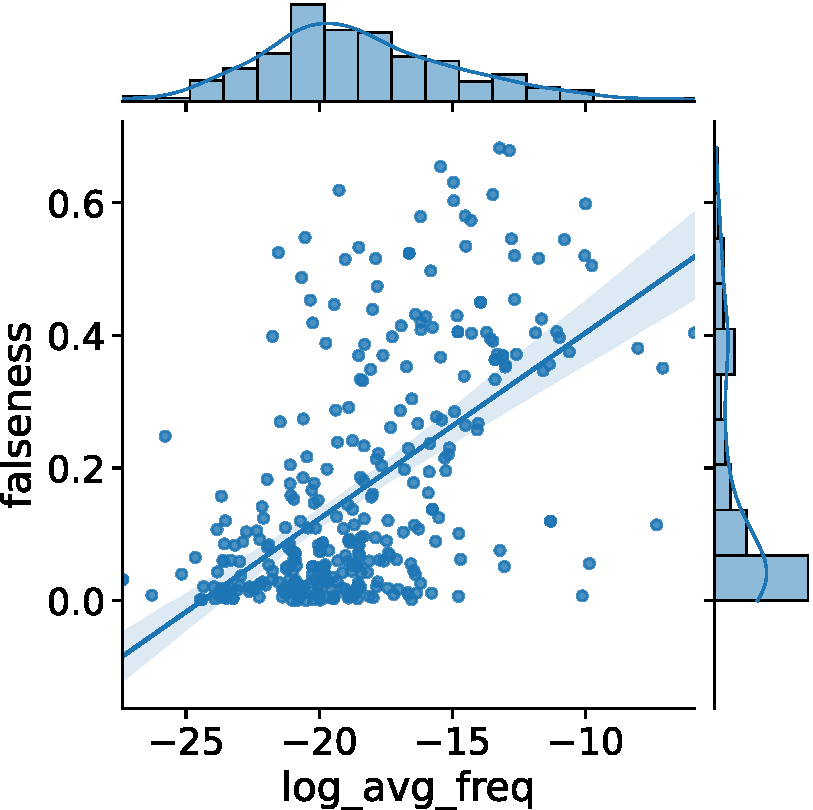
\includegraphics[width=\linewidth]{figures/UBAN_correlation_es_pt_falseness_logfreq_big.pdf}
    \end{subfigure}\begin{subfigure}{0.5\textwidth}\centering
    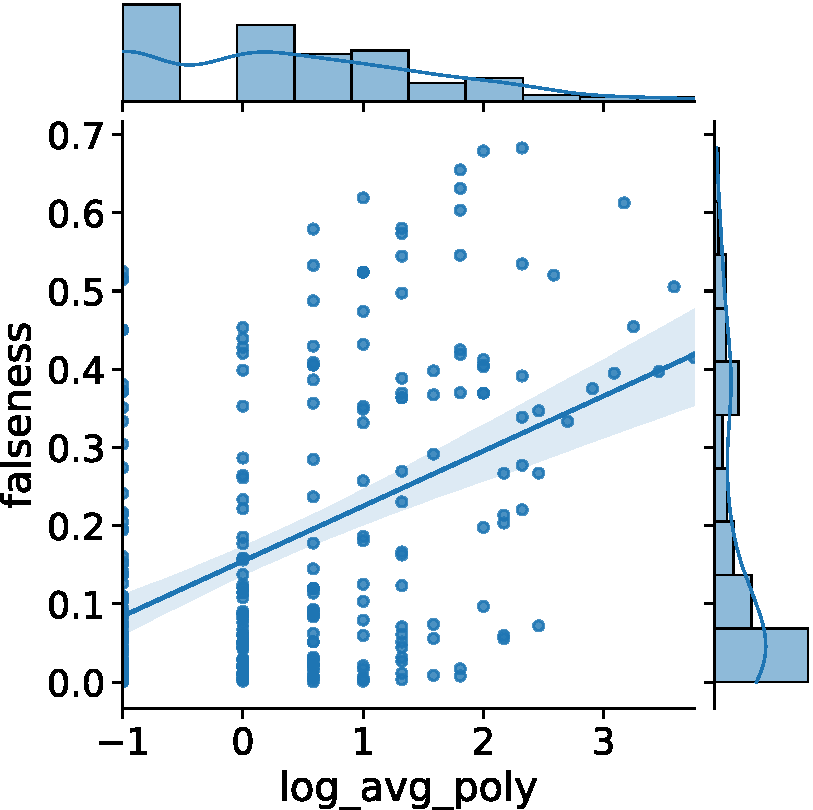
\includegraphics[width=\linewidth]{figures/UBAN_correlation_es_pt_falseness_logpoly_big.pdf}
    \end{subfigure}
\caption{Falseness correlation with log-frequency and log-polysemy for Spanish-Portuguese.\label{fig:scatter2}}
\end{figure}\clearpage



We then try to find a function that describes in more precise terms the relationship between frequency and meaning shift, by fitting a polynomial curve of the following form:

\begin{equation}
    \text{falseness} = a * (\log_{10}(\text{freq}))^b + c
\end{equation}
where $a$, $b$ and $c$ are the parameters of the function. 

Using the polynomial class of functions allows us flexibility in understanding the nature of the relationship (positive or negative, according to the sign of the main coefficient $a$), and its magnitude as measured by the size of the main coefficient and by the power coefficient $b$, while still being restrictive enough to facilitate computation using the limited training vocabulary in our dataset.

The complete list of the computed coefficients is shown in Table~\ref{tab:freq-coeffs}. We find that for most language pair there is a positive and superlinear relationship between the log-frequency score and the degree of falseness, with coefficients $b$ generally close to 1, for all Romance language pairs, except for Romanian. For Romanian the power coefficients are higher across language pairs, associated with lower main coefficients, but their values less stable and less reliable, which we attribute to the lower coverage and quality of frequency scores, as well as to the inclusion of all cognates without filtering just the false friends. For pairs involving English, the algorithm generally fails to find a consistent relationship between the variables: it converges slower and is less stable, producing power coefficients that are very low, essentially resulting in an equation where the frequency variable is negligible.

\begin{table}
    \begin{tabular}{l S[table-format=3.4]S[table-format=1.3]S[table-format=-3.2]  S[table-format=3.4]S[table-format=1.4]S[table-format=-3.3]}
    \lsptoprule
        & \multicolumn{3}{c}{Es} & \multicolumn{3}{c}{Pt}\\\cmidrule(lr){2-4}\cmidrule(lr){5-7}
        & {$a$} & {$b$} & {$c$} & {$a$} & {$b$} & {$c$} \\\midrule
        Es &  &  &  & 0.04 & 1.27 & -0.01\\                    
        Pt & 0.04 & 1.30 & -0.03 &  &  & \\                    
        It & 0.06 & 1.09 & -0.07 & 0.08 & 0.80 & -0.05\\       
        Fr & 0.10 & 0.86 & -0.12 & 0.07 & 0.91 & -0.03\\       
        Ro & 0.007 & 1.41 & 0.06 & 0.006 & 1.41 & 0.07\\       
        En & 2.90 & 0.12 & -3.10 & 201.8 & 0.001 & -201.8\\\midrule 
           & \multicolumn{3}{c}{It} & \multicolumn{3}{c}{Fr}\\\cmidrule(lr){2-4}\cmidrule(lr){5-7}
           & {$a$} & {$b$} & {$c$} & {$a$} & {$b$} & {$c$} \\\midrule
        Es & 0.06 & 1.12 & -0.08      & 0.25 & 0.58 & -0.31\\     
        Pt & 0.04 & 1.07 & -0.01      & 0.07 & 0.96 & -0.03\\     
        It &  &  &                    & 0.05 & 1.17 & -0.004 \\    
        Fr & 0.10 & 0.82 & -0.09      &  &  &        \\            
        Ro & 0.01 & 1.06 & 0.05       & 0.004 & 1.86 & 0.07\\      
        En &493.1 & 0.05 & -493.1 & 675.5 & 0.0005 & -675.6\\\midrule
            & \multicolumn{3}{c}{Ro} & \multicolumn{3}{c}{En}\\\cmidrule(lr){2-4}\cmidrule(lr){5-7}
            & {$a$} & {$b$} & {$c$} & {$a$} & {$b$} & {$c$}\\\midrule
        Es  & 0.0003 & 3.11 & 0.08 & 580.3 & 0.0005 & -580.4 \\
        Pt  & 0.0002 & 2.85 & 0.08 & 528.9 & 0.0005 & -528.9 \\
        It  & 0.0003 & 3.17 & 0.08 & 463.8 & 0.0006 & -463.8  \\
        Fr  & 0.0001 & 3.58 & 0.09 & 579.6 & 0.0005 & -579.7\\
        Ro  &  &  &  & 144.3 & 0.0007 & -144.2\\ 
        En  & 257.2 & 0.0003 & 257.1 &  &  &  \\
        \lspbottomrule
    \end{tabular}
    \caption{Optimal coefficients of polynomial describing function between frequency and falseness as $\text{falseness} = a * (\log_{10}(\text{freq}))^b + c$.\label{tab:freq-coeffs}}
\end{table}

It is interesting to compare our results with those of \citet{hamilton-etal-2016-diachronic}, where the authors observe an inverse correlation between frequency and meaning shift: the more frequent words tend to change their meaning more slowly. Our experiments are set up to describe the phenomenon of semantic change from the opposite direction, measuring the expected frequency of a word that has undergone semantic change, and show the opposite effect: we find a positive relation -- words that have diverged more in meaning tend to be more frequent.


\subsection{Word polysemy and semantic divergence}
For measuring \textit{polysemy}, we make use of WordNet. In this way, the polysemy of a word can be defined as the number of synsets that it is part of in WordNet. As before, we have to exclude Romanian since it is not supported in WordNet (we assign a default polysemy score of $0$ to all Romanian words). The polysemy score of a cognate pair is computed as the average between the polysemy scores of the two words involved.


We perform similar experiments for polysemy, correlating the average degree of polysemy of the words in a cognate pair to the falseness of the pair, with frequency as a control variable. The obtained correlations, shown in Table \ref{tab:poly-corr}, are noteworthy for most language pairs, with values as high as $0.47$. Figure \ref{fig:scatter2} shows the relationship between log-polysemy and falseness, which displays a clear linear trend.


\begin{table}
    \begin{tabular}{l *{6}{S[table-format=-1.3]} }
\lsptoprule
        & {Es} & {Pt} & {It} & {Fr} & {Ro} & {En} \\ \midrule
        Es &  & 0.404 & 0.342 & 0.336 & 0.072 & 0.286 \\
        Pt & 0.461 &  & 0.363 & 0.427 & -0.004 & 0.305 \\
        It & 0.305 & 0.383 &  & 0.412 & 0.019 & 0.087 \\
        Fr & 0.341 & 0.413 & 0.479 &  & -0.051 & 0.184 \\
        Ro  & 0.093 & -0.01 & -0.011 & -0.049 &  & -0.016 \\ 
        En & 0.429 & 0.37 & 0.087 & 0.301 & -0.062 &  \\
\lspbottomrule
    \end{tabular}
    \caption{Correlations of polysemy with falseness, controlling for frequency.\label{tab:poly-corr}}
\end{table}

For Romance languages (with some isolated exceptions for pairs involving Romanian), polysemy proves to be strongly positively correlated with falseness, suggesting words which have undergone more semantic shift tend to be more polysemous. Previous studies \citep{hamilton-etal-2016-diachronic} have found a positive relationship between polysemy and semantic change from the opposite perspective, showing that more polysemous words seem to suffer more semantic shift. 

We further compute a polynomial that approximates the relationship between the log-polysemy score and falseness, following the general form:
\begin{equation}
    \text{falseness} = a * \log_2(\text{polysemy})^b + c
\end{equation}
where $a$, $b$ and $c$ are the coefficients to be found. In this case, all polysemy scores are non-negative integers. For words not found in WordNet, we replace the log-polysemy score with zeroes.

In the case of polysemy, we find a sublinear relationship between log-po\-ly\-semy and falseness. Coefficients are listed in Table \ref{tab:poly-coeffs}.
The main coefficients are always positive, with the exception of one language pair (Romanian-English), and the power $b$ is usually in the interval $(0.5, 1)$, for all languages, with the exception of Italian-English and several language pairs involving Romanian, where they are higher. We expect the results for Romanian to be less reliable in this case as well, since we lack polysemy scores for Romanian entirely (polysemy scores for language pairs involving Romanian rely entirely on the other language in the pair). In general, scores are more stable than in the case of the frequency-falseness law, including for English and for Romanian.

The positive relationship between falseness and both frequency and polysemy suggest words that have undergone semantic change tend to become more frequent as well as more polysemous, proportional to the degree of semantic shift, maintaining a consistent pattern across language pairs, especially among core Romance languages (Italian, French, Spanish, Portuguese). Overall, the higher power coefficients for frequency in relation to falseness (as compared to the case of polysemy) suggest that more pronounced shifts in meaning are associated with increases in frequency, as compared to polysemy where the meaning divergence associated with a change in polysemy is relatively milder. The more uniform coefficients in the laws relating polysemy and falseness across languages, as well as the higher partial correlation scores for polysemy, suggest a more consistent pattern of association between semantic divergence and polysemy (as compared to frequency).

\begin{table}
    \begin{tabular}{l *{2}{S[table-format=1.3]S[table-format=1.2]S[table-format=1.2]}  S[table-format=-1.3]S[table-format=1.2]S[table-format=1.2]}
    \lsptoprule
        & \multicolumn{3}{c}{Es} & \multicolumn{3}{c}{Pt} & \multicolumn{3}{c}{It}\\\cmidrule(lr){2-4}\cmidrule(lr){5-7}\cmidrule(lr){8-10}
        & {$a$} & {$b$} & {$c$} & {$a$} & {$b$} & {$c$} & {$a$} & {$b$} & {$c$}\\
        \midrule
        Es &      &      &      & 0.10 & 0.99 & 0.11 & 0.11 & 0.78 & 0.11  \\ 
        Pt & 0.10 & 0.93 & 0.10 &      &      &      & 0.07 & 1.02 & 0.11  \\ 
        It & 0.10 & 0.56 & 0.12 & 0.07 & 0.73 & 0.11 &     &     &      \\ 
        Fr & 0.07 & 0.81 & 0.12 & 0.05 & 0.93 & 0.14 & 0.07 & 0.79 & 0.13  \\ 
        Ro & 0.03 & 0.62 & 0.07 & 0.02 & 0.82 & 0.07 & 0.01 & 1.91 & 0.09  \\  
        En & 0.13 & 0.66 & 0.19 & 0.10 & 0.43 & 0.23 & 0.0004 & 3.60 & 0.32\\
        \midrule
        & \multicolumn{3}{c}{Fr} & \multicolumn{3}{c}{Ro} & \multicolumn{3}{c}{En}\\\cmidrule(lr){2-4}\cmidrule(lr){5-7}\cmidrule(lr){8-10}
        & {$a$} & {$b$} & {$c$}  & {$a$} & {$b$} & {$c$} & {$a$} & {$b$} & {$c$}\\\midrule
        Es & 0.08 & 0.72 & 0.14  & 0.02 & 0.86 & 0.07 & 0.07 & 0.75 & 0.26 \\
        Pt & 0.06 & 0.83 & 0.15  & 0.02 & 0.55 & 0.07 & 0.06 & 0.69 & 0.27\\
        It & 0.06 & 0.76 & 0.16  & 0.01 & 1.26 & 0.08 & 0.0004 & 3.60 & 0.32  \\
        Fr &      &      &       & 0.004 & 2.23 & 0.08 & 0.02 & 0.98 & 0.30 \\
        Ro & 0.004 & 2.18 & 0.09 &       &     &     & -0.007 & 0.27 & 0.19  \\
        En & 0.06 & 0.78 & 0.25  & 0.0001 & 4.99 & 0.16 &  &  &  \\ 
        \lspbottomrule
    \end{tabular}
    \caption{Optimal coefficients of polynomial describing function between polysemy and falseness as $\text{falseness} = a * (\log_2(\text{poly}))^b + c$.\label{tab:poly-coeffs}}
\end{table}

\subsection{Semantic fields of true cognates}

In this final subsection, we present a brief qualitative analysis of true cognates across the Romance languages -- the words that have preserved their meaning from their Latin etymon to the present day meaning, comparatively across languages. We use clustering methods to extract clusters of true cognates that can be interpreted to represent the different semantic fields of the words that have preserved their meaning throughout time. We show these examples as an initial attempt to better understand how the semantic change of words varies across semantic fields, comparatively across languages which diverged from Latin (based on the simplifying assumption that the extracted true cognates are inherited words) in different moments in history and different geographical, political and cultural contexts.   

In order to obtain semantic clusters for each language, we first select the true cognates from our list of cognate sets, for language pairs consisting of Latin and a Romance language, using our algorithm (by selecting word pairs with null falseness scores). For each Romance language, we collect the vector representations of the extracted words in the corresponding embedding space. We then apply $k$-means clustering on this set of points to obtain 10 clusters, based on the cosine distance between the vectors, approximating the semantic distance between the extracted true cognates. For each resulted cluster, we find the centroid point, which we approximate with its closest word in the embedding space of that language (whether the resulting word is in our cognate set or not). In the end, we are left with 10 semantic clusters for each Romance language, each represented by a centroid word. 

%We show the resulting clusters in Table \ref{tab:semantic_fields}. Each cell in the table represents one cluster, containing the centroid word, along with each word's translation in English (where they are meaningful), in decreasing order of the number of words in the cluster. Since not all centroid words are meaningful or representative, we also include on the following rows row for each cluster 4 representative words chosen manually from the true cognates belonging to the cluster, along with their translations. 

We show the resulting clusters in Appendix~\ref{sec:07:appendix}. The first element of each line represents one cluster, containing the centroid word (rendered in bold letters), along with each word's translation in English (where they are meaningful), in decreasing order of the number of words in the cluster. Since not all centroid words are meaningful or representative, we also include on the same line, for each cluster, 4 representative words chosen manually from the true cognates belonging to the cluster, along with their translations.

It is interesting to see that there are a few semantic fields that occur consistently in each language: terms related to morality and justice, to medicine, and to chemistry or abstract mathematics. Some clusters are specific to certain domains that do not occur in each language, such as foods (in Portuguese), mechanical terms (in Portuguese and Romanian), or religious terms (in Romanian).

We should note a limitation of the method used to obtain the semantic clusters, stemming from the representation of Latin words. All word embedding representations used in this study were based on pre-trained FastText embeddings trained on Wikipedia \citep{cognatesuban:conneau2017word}, including Latin embeddings. The uniformity of the text genres and topics across languages is in general an advantage to obtaining comparable embedding spaces, but in the case of Latin, the use of Latin Wikipedia, which consists of translated texts from other languages, might bias representations away from the original usages of the words in Latin, and towards their usages in the modern languages the texts were translated from, and consequently affect the detection of true cognates in relation to Latin. This drawback could be mitigated by using a corpus of original Latin texts instead for building the embeddings.

\section{Conclusions}
\label{section:conclusions}

In this chapter, we proposed a method for computing the semantic divergence of cognates across languages, and showed how it can be used for computing language similarity, for measuring cross-lingual semantic change synchronically, as well as for practical applications including false friend detection and correction. 

We defined a cross-lingual word similarity measure based on word embeddings and extended the pairwise metric to compute the semantic divergence across languages. Our results showed that Spanish and Portuguese are the closest languages, while Romanian is most dissimilar from Latin, possibly because it developed far from the Romance kernel. Furthermore, clustering the Romance languages based on the introduced semantic divergence measure resulted in a hierarchy that is consistent with the generally accepted tree of languages. When further including English in our experiments, we noticed that, even though most Latin words that entered English are probably borrowings (as opposed to inherited words), its similarity to Latin is close to that of the modern Romance languages. Our results shed some light on a new aspect of language similarity, from the point of view of cross-lingual semantic change.

We further showed how the introduced measures can be used for a practical application, and proposed a method for detecting false friends from cognate word pairs, distinguishing between two categories: hard false friends and soft false friends. Additionally, we built and made freely available a database of false friends in six languages, and evaluated it against WordNet and against a manually curated dataset of false friends, obtaining state of the art results.
To the best of our knowledge, the published database is the largest public resource of its kind, both in terms of number of covered word pairs and considered languages. Additionally, the proposed method can be used to generate or detect pairs of false friends for any pair of languages, without requiring expensive manual work or dictionaries, but only large monolingual corpora to train word embeddings on, and small bilingual dictionaries to perform embedding space alignments.

\begin{sloppypar}
We also proposed an algorithm for automatically correcting false friends, which to our knowledge is the first attempt in this direction. 
Along with false friends pairs, we published a falseness score for each pair, which can be used to customize the sensitivity to difference in meaning that defines a pair of false friends according to the application. We believe this resource can be very valuable for language learners, for example by incorporating false friends pairs in a tool to aid with language acquisition or text comprehension for non-natives, as well as for machine translation or other applications using natural language processing in a multilingual setting.
\end{sloppypar}

The unsupervised nature of the proposed algorithm also has the advantage of a high coverage of the vocabulary, unlike dictionary-based methods, which are prone to becoming outdated as language evolves. One disadvantage of our embedding-based algorithm is the lack of distinction between different senses of the same word. In the future it would be interesting to continue the study in the direction of considering also context-specific senses of words, in order to be able to better handle partial false friends, which are pairs of cognates which share meaning in some contexts and not in others. In the case of corrections as well, the method using word embeddings could be extended to provide false friend correction suggestions in a certain context (possibly by using the word embedding model to predict the appropriate word in a given context).

In the fourth section, we showed a new perspective for studying semantic change: comparing meaning of cognate words across languages.
We showed how frequency and polysemy relate to semantic shifts of cognates across languages, demonstrating that both the frequency and polysemy of cognates positively correlate with their cross-lingual semantic shift, suggesting that semantic change, in the case of cognates, drives words to be both more frequent and more polysemous. Moreover, we found concrete functions that best approximate these relationships according to a power law, thus taking the first steps towards formulating statistical laws of cross-lingual semantic change. 

In the future, including the proto-word in the analysis relating semantic shift to word properties (in this case, the Latin etymon) may give further insight into how cognates change their meaning, as well as allow the exploration of the reverse effect, that of the influence of word properties (frequency, polysemy, etc.) on the magnitude of the subsequent semantic shift.
 Exploring alternative methods for obtaining multilingual word representations (through choosing a different training corpus or reducing the noise induced by embedding space alignment) would help to further strengthen our conclusions on multilingual language phenomena related to semantic change. Additionally, it would be interesting to further explain these correlations, as well as study other hypothesized laws of semantic change in a multilingual setting (such as the law of differentiation or parallel change, or the law of prototypicality), extending the study to other language families beyond the Romance cluster. 
 
 \appendixsection{Clusters of true cognates per language: centroids, representative words, and English translations.}\label{sec:07:appendix}
 
 \begin{itemize}[leftmargin=*]\sloppy
	\item Spanish
	\begin{itemize}
		\item \textbf{amoralidad (amorality)}, abstinente (abstinent), bueno (good), compasion (compassion), profeta (prophet)
		\item \textbf{--}, ébano (ebony), equino (equine), playa (beach), estatuaria (statuary)
		\item \textbf{reversibilidad (reversibility)}, abstracción (abstraction), ecuación (equation), exceso (excess), inductivo (inductive)
		\item \textbf{contrar (counter)}, cazar (hunt), devastar (devastate), encender (ignite), salir (leave)
		\item \textbf{cuotificación (quota)}, colectivo (collective), declaración (declaration), institución (institution), juez (judge)
		\item \textbf{hiposalivación (hyposalivation)}, artrítico (arthritic), irritación (irritation), reumatismo (rheumatism), ulceración (ulceration)
		\item \textbf{inmoralidad (immorality)}, abominable (abominable), disidente (dissident), indecente (indecency), perversidad (perversion)
		\item \textbf{embrazadura (embracing)}, cicatriz (scar), hueso (bone), rotura (break), vibrar (vibrate)
		\item \textbf{ahúma (smoke)}, bálsamo (balsam), freir (fry), arroz (rice), huevo (egg)
		\item \textbf{higroscópico (hygroscopic)}, cáustico (caustic), evaporar (evaporate), fósforo (phosphorus), ópalo (opal)
	\end{itemize}
	\pagebreak
	\item Portuguese
	\begin{itemize}
		\item \textbf{--}, ébano (ebony), cobra (snake), hipódromo (hippodrome), vaqueiro (cowboy)
		\item \textbf{pessoalização (personalization)}, acessível (accessible), conciliação (conciliation), educação (education), monarquia (monarchy) 
		\item \textbf{imoralidade (immorality)}, abjeto (abject), dissidente (dissident), incriminar (incriminate), promíscuo (promiscuous)
		\item \textbf{amoralidade (amorality)}, admiração (admiration), autêntico (authentic), generosidade (generosity), monogamia (monogamy)
		\item \textbf{pessoalizar (personalize)}, causar (cause), decidir (decide), justificar (justify), sugerir (suggest)
		\item \textbf{pneumogástrico (pneumogastric)}, atrofia (atrophy), inflamação (inflammation), irritação (irritation), tosse (cough)
		\item \textbf{irrotacional (irrotational)}, dispositivo (device), oscilação (oscillation), esférico (spherical), vibrar (vibrate)
		\item \textbf{sêmola (semolina)}, agricultura (agriculture), bovino (bovine), forno (oven), suco (juice)
		\item \textbf{--}, abstração (abstraction), convergir (converge), infinito (infinite), qua\-drilátero (quadrilateral)
		\item \textbf{anidrita (anhydrite)}, alumínio (aluminium), emoliente (emollient), insolúvel (insoluble), viscoso (viscous)
	\end{itemize}
	\item Italian
	\begin{itemize}
		\item \textbf{moralizzare (moralize)}, apprendere (learn), cooperare (cooperate), evacuare (evacuate), presentare (present)
		\item \textbf{--}, albore (dawn), complesso (complex), lupo (wolf), tempo (time)
		\item \textbf{giovevole (beneficial)}, austero (austere), circospetto (circumspect), delicato (delicate), delinquente (delinquent)
		\item \textbf{commiserazione (commiseration)}, affettazione (affectation), catastrofe (catastrophe), inspirazione (inspiration), emozione (emotion)
		\item \textbf{--}, accelerazione (acceleration), ciclico (cyclic), deduttivo (deductive), eccesso (excess)
		\item \textbf{espromissione (indivisibile)}, anticipazione (anticipation), comunicazi\-o\-ne (communication), creazione (creation), emanazione (emanation)
		\item \textbf{ulcerazione (ulceration)}, abortivo (abortion), cicatrice (scar), glaucoma (glaucoma), irritazione (irritation)
		\item \textbf{insaporimento (flavor)}, coagulare (coagulate), fermentare (fermen), masticare (chewing), vegetare (vegetate)
		\item \textbf{carbonatazione (carbonation)}, asfalto (asphalt), cristallino (crystalline), corrodere (corrode), ossidiana (obsidian)
		\item \textbf{stilofaringeo (stylopharyngeal)}, vescica (bladder), coronale (coronal), polmone (lang), ventrale (ventral)
	\end{itemize}
	\item French
	\begin{itemize}
		\item \textbf{amoralité (amorality)}, arrogance (arrogance), conjugal (conjugal), émotion (emotion), inflexible (inflexible)
		\item \textbf{--}, ambassade (embassy), convention (convention), éducation (education), gymnastique (gymnastics)
		\item \textbf{apppliquer (apply)}, menacer (threat), combiner (combine), extraire (extract), jouer (play)
		\item \textbf{--}, apostrophe (apostrophe), déductif (deductive), indication (indication), oeil (eye)
		\item \textbf{bénédictionnaire (blessed)}, autographe (autograph), décalogue (decalogue), martyr (martyr), nobiliaire (nobiliary)
		\item \textbf{--}, cyclique (cyclic), convexité (convexity), intersection (intersection), saturation (saturation)
		\item \textbf{chapelure (breadcrumbs)}, chaud (warm), crème (cream), macération (maceration), spatule (spatula)
		\item \textbf{entérotoxémie (enterotoxemia)}, clinique (clinical), convalescent (convalesent), immunité (immunity), médication (medication)
		\item \textbf{testiculaire (testis)}, atrophie (atrophy), genou (knee), estomac (stomach), vertébré (vertebra)
		\item \textbf{silicique (silicic)}, gélatine (gelatine), caustique (caustic), corroder (corrode), pigment (pigment)
	\end{itemize}
	\item Romanian
	\begin{itemize}
		\item \textbf{grăunțoasă (grainy)}, aramă (copper), cuc (cuckoo), plajă (beach), suc (juice)
		\item \textbf{senilitate (senility)}, anticipație (anticipation), enormitate (enormity), fascinație (fascination), intrigă (intrigue)
		\item \textbf{--}, mecanic (mechanical), accesibil (accessible), arc (arc), fluctuație (fluctuation)
		\item \textbf{incognoscibil (unknowable)}, adorabil (adorable), afective (affective), inaccesibil (inaccessible), invizibil (invisible)
		\item \textbf{limfadenopatie (lymphadenopathy)}, apoplecie (apoplecia), cicatrice (scar), letal (lethal), coagula (clot)
		\item \textbf{--}, beneficiar (beneficiary), comitet (committee), învăța (learn), proprietar (owner)
		\item \textbf{condamnabil (condemnable)}, calomnia (slander), discrimina (discriminate), nega (deny), infidel (unfaithful)
		\item \textbf{triclorurii (trichloride)}, aprinde (ignite), compozit (composite), cristalin (crystalline), cuaternar (quaternary)
		\item \textbf{pantocrator (pantocrator)}, altar (altar), cruce (cross), exorcist (exorcist), sacrilegiu (sacrilege)
		\item \textbf{perifraze (periphrases)}, apostrof (apostrophe), impersonal (impersonal), intranzitiv (intransitive), predicativ (predicative)
	\end{itemize}
\end{itemize}
 
 
\section*{Acknowledgements}
\begin{sloppypar}
We thank the reviewers for their helpful and constructive comments.
This work was supported by a grant of the Romanian Ministry of Education and Research, CNCS - UEFISCDI,  CoToHiLi project, number PN-III-P4-ID-PCE-2020-1544, within PNCDI III.
\end{sloppypar}

\section*{Abbreviations}
\begin{tabularx}{.5\textwidth}[t]{@{}lQ@{}}
BLI & Bilingual Lexicon Induction \\
Es & Spanish \\
FF & false friends \\
freq & frequency \\
Fr & French \\
It & Italian \\
La & Latin \\
poly & polysemy\\
\end{tabularx}\begin{tabularx}{.5\textwidth}[t]{@{}lQ@{}}
Pt & Portuguese \\
Ro & Romanian \\
Ro & Romanian \\
UPGMA & Unweighted pair group method with arithmetic mean \\
WN & WordNet \\
\end{tabularx}

{\sloppy\printbibliography[heading=subbibliography,notkeyword=this]}
\end{document}
